\chapter{Supplementary figures}
\label{app:figures}

% 3 - LOCUS CHAPTER

\begin{figure}
	\centering
	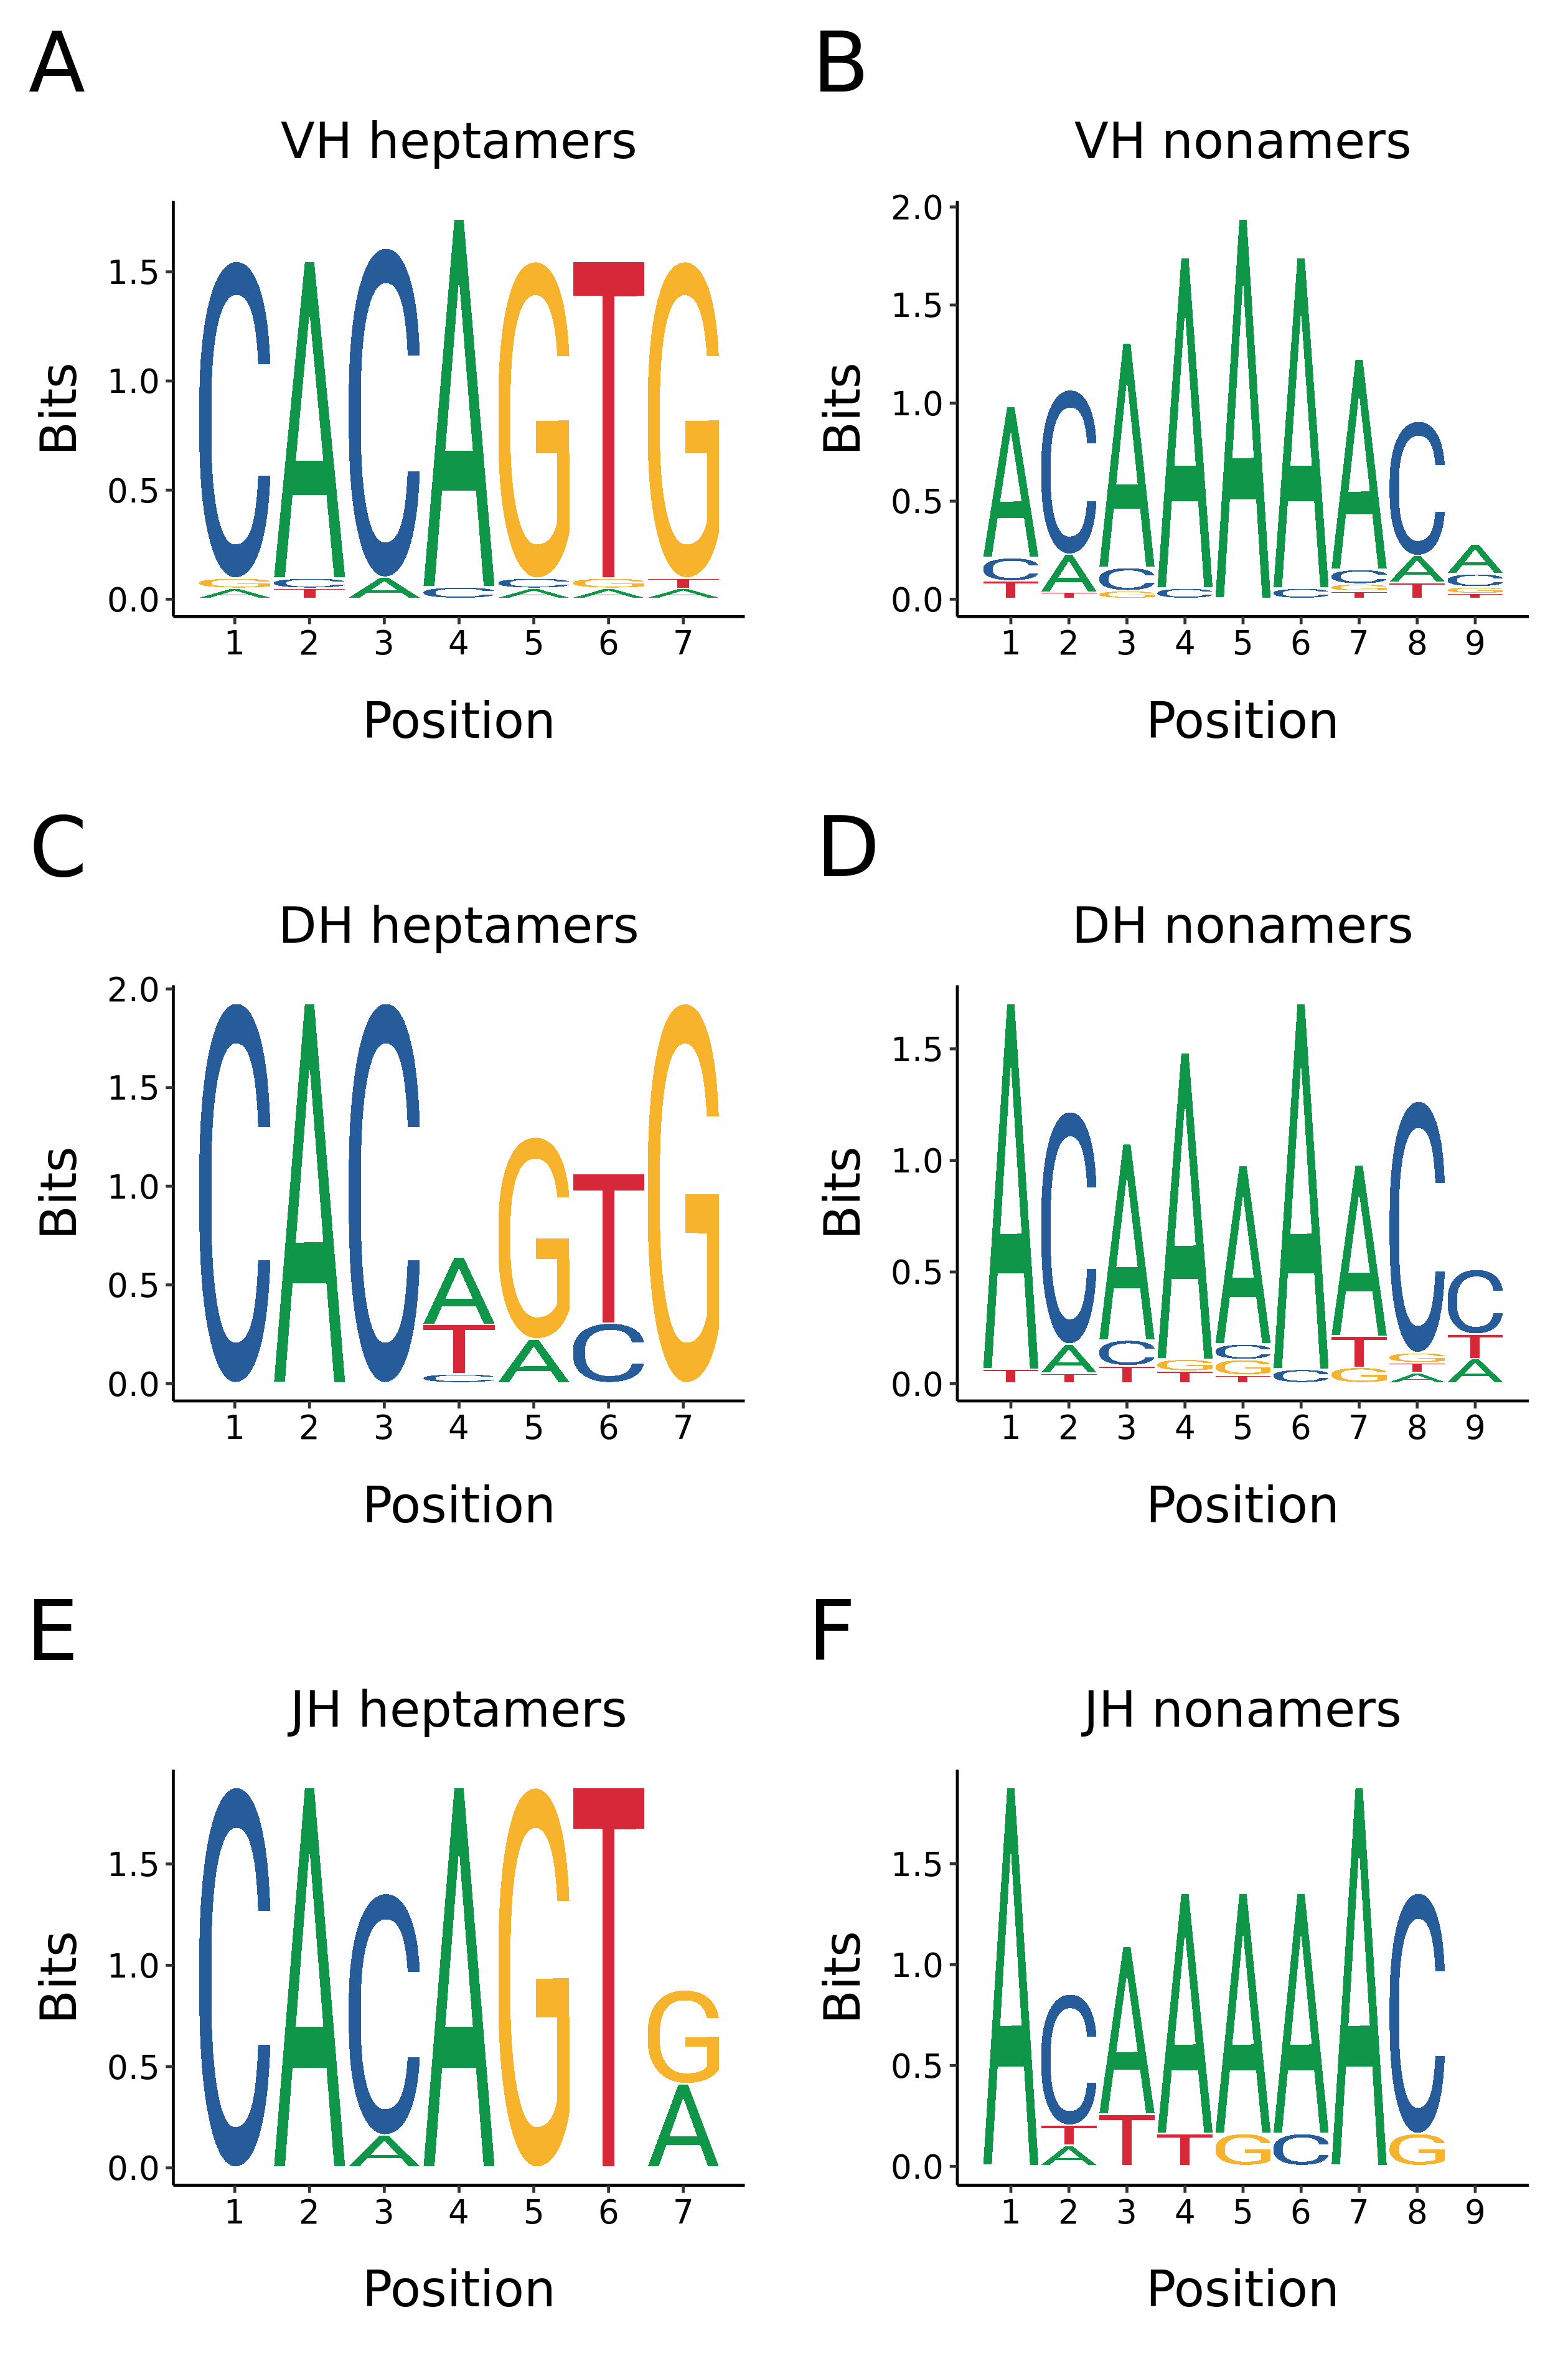
\includegraphics[width=0.9\textwidth]{_Figures/png/nfu-rss-seqlogo-sep}
	\caption[\Nfu recombination signal sequences by segment type]{\textbf{\Nfu recombination signal sequences by segment type:} Sequence composition of conserved heptamer (A,C,E) and nonamer (B,D,F) sequences from \Nfu heavy-chain RSSs associated with \vh (A,B), \dh (C,D) or \jh (E,F) gene segments.}
	\label{fig:nfu-rss-seqlogo-sep}
\end{figure}

\begin{figure}
	\centering
	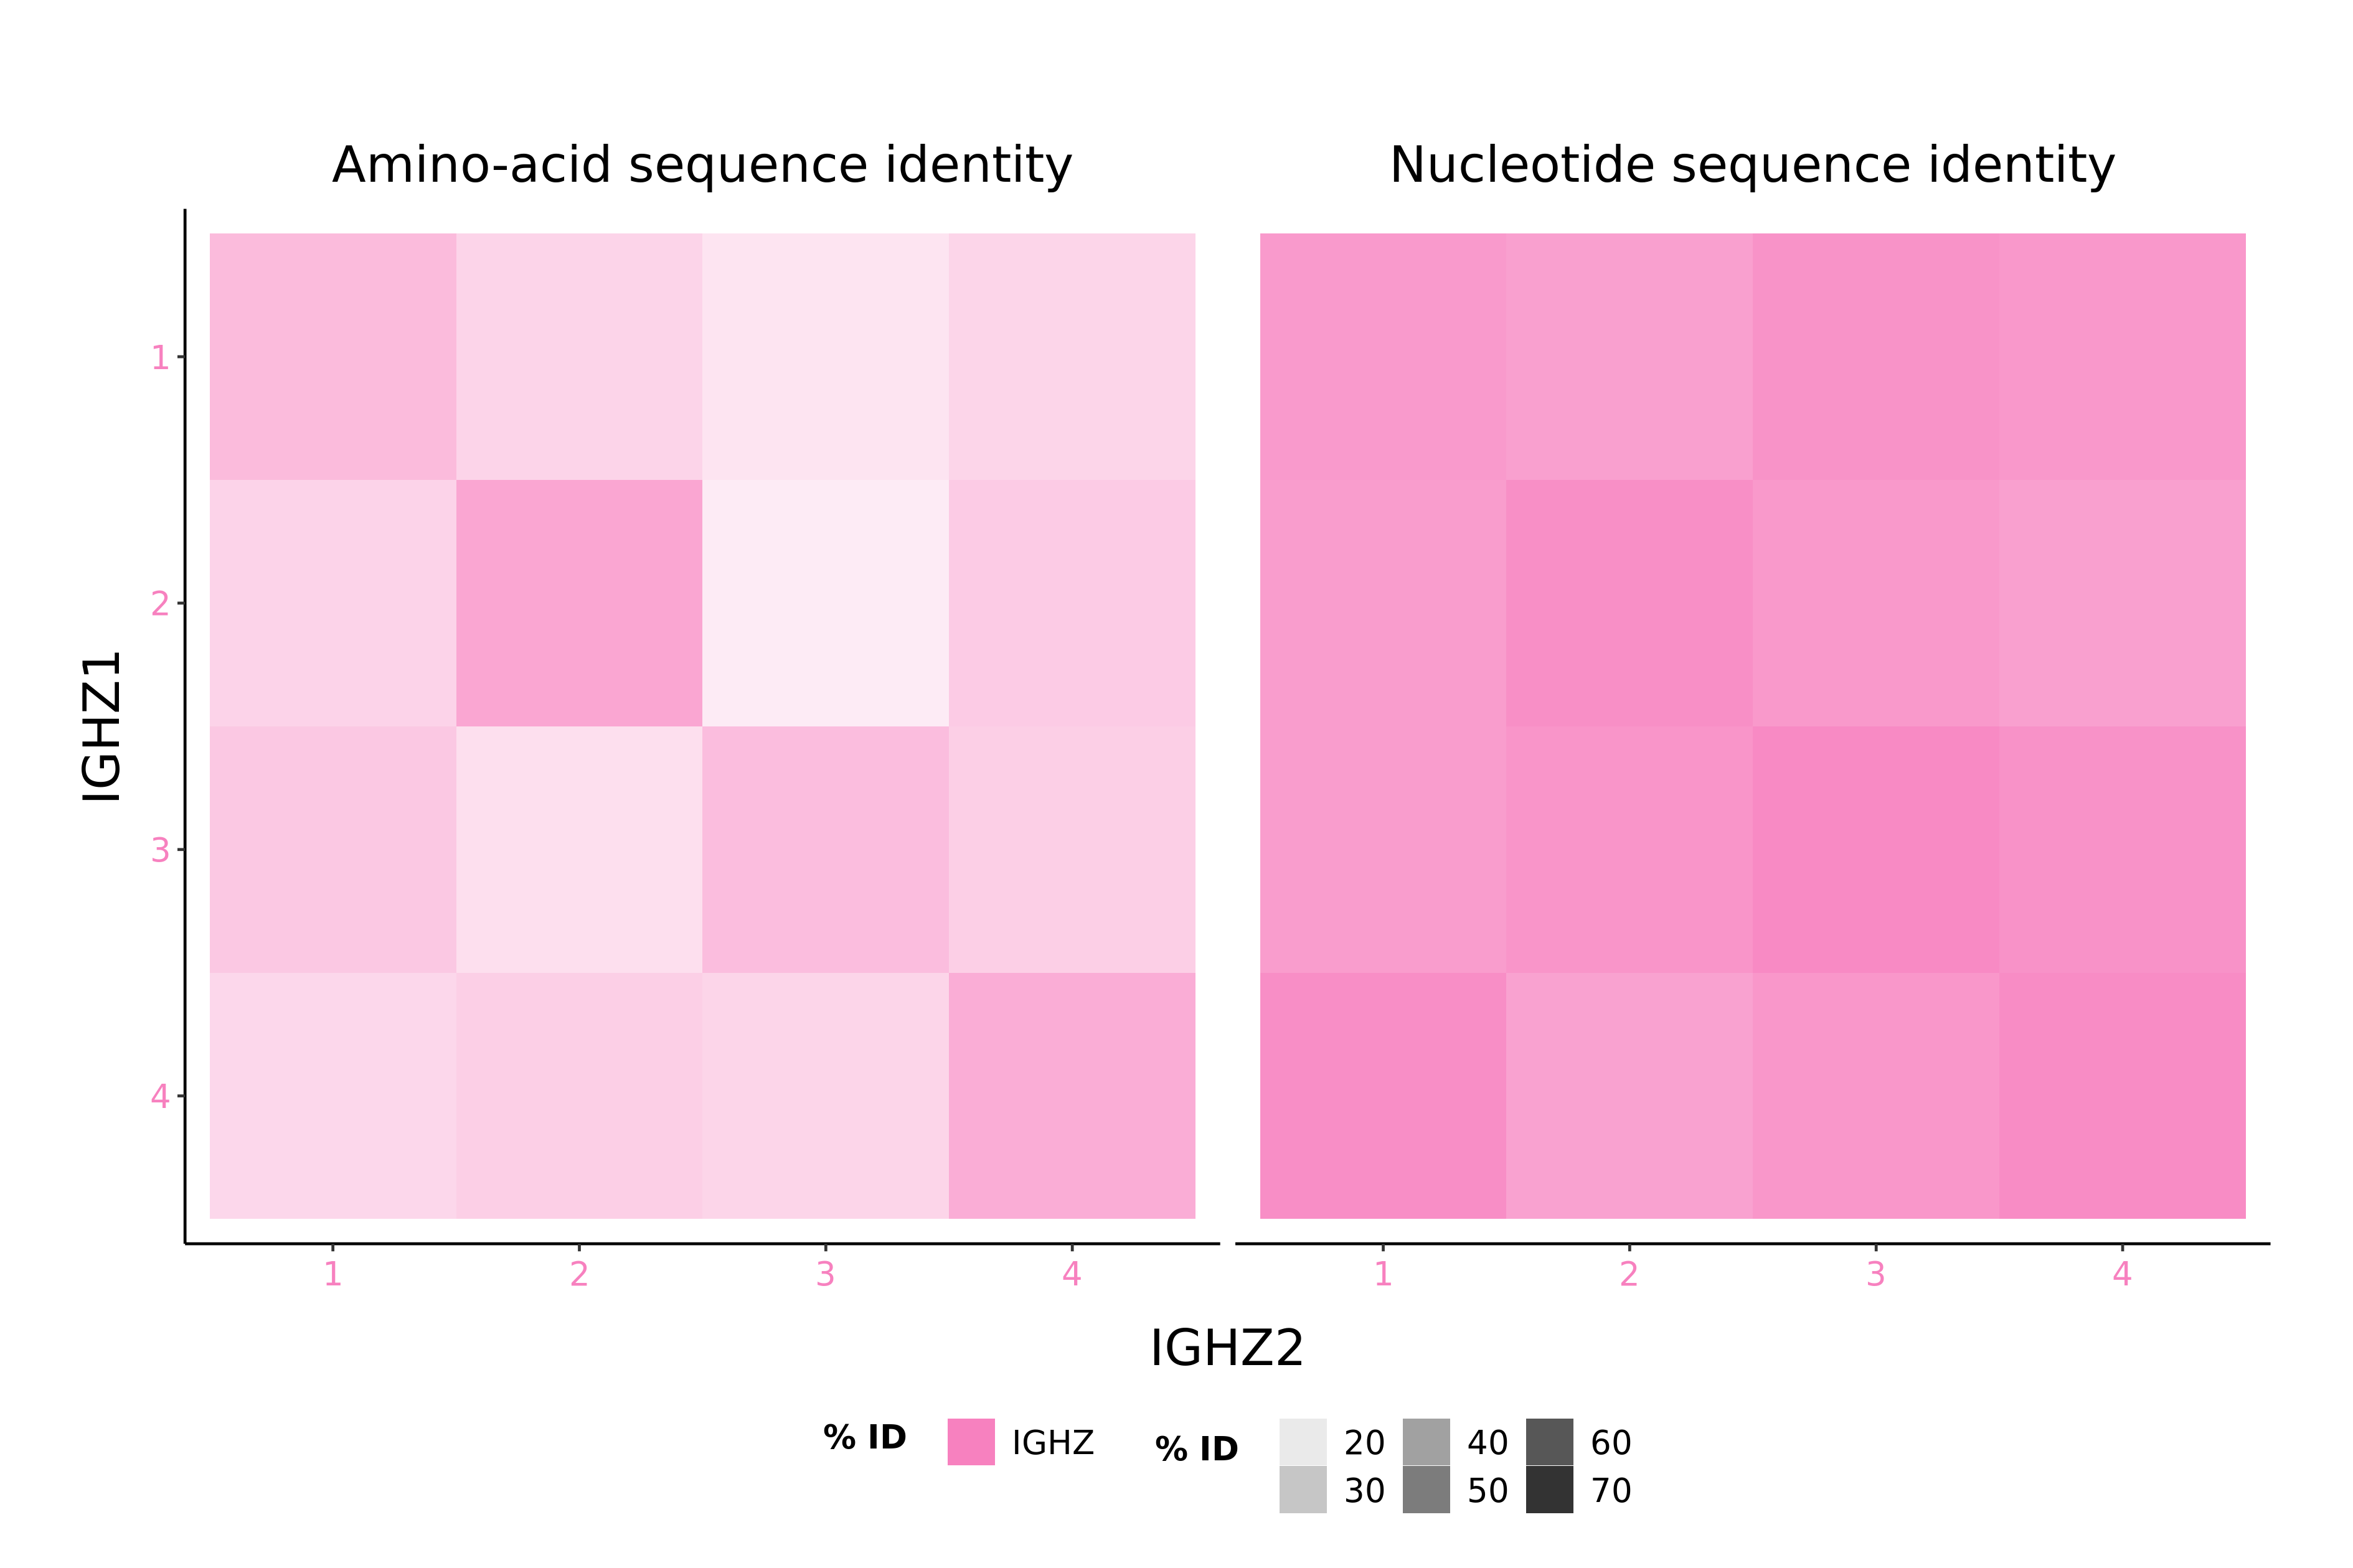
\includegraphics[width=0.8\textwidth]{_Figures/png/xma-new-cz-aln}
	\caption[Sequence similarity between \igh{Z} constant-regions in \Xma]{\textbf{Sequence similarity between \igh{Z} constant-regions in \Xma:} Heatmap of percentage sequence identity between amino-acid (right) and nucleotide (left) sequences of \cz{} exons from the two \Xma \igh{Z} constant regions, calculated using pairwise Needleman-Wunsch global alignments.} % TODO: Combine isotype and identity legends
	\label{fig:xma-cz-aln}
\end{figure}

	\begin{figure}
	\centering
	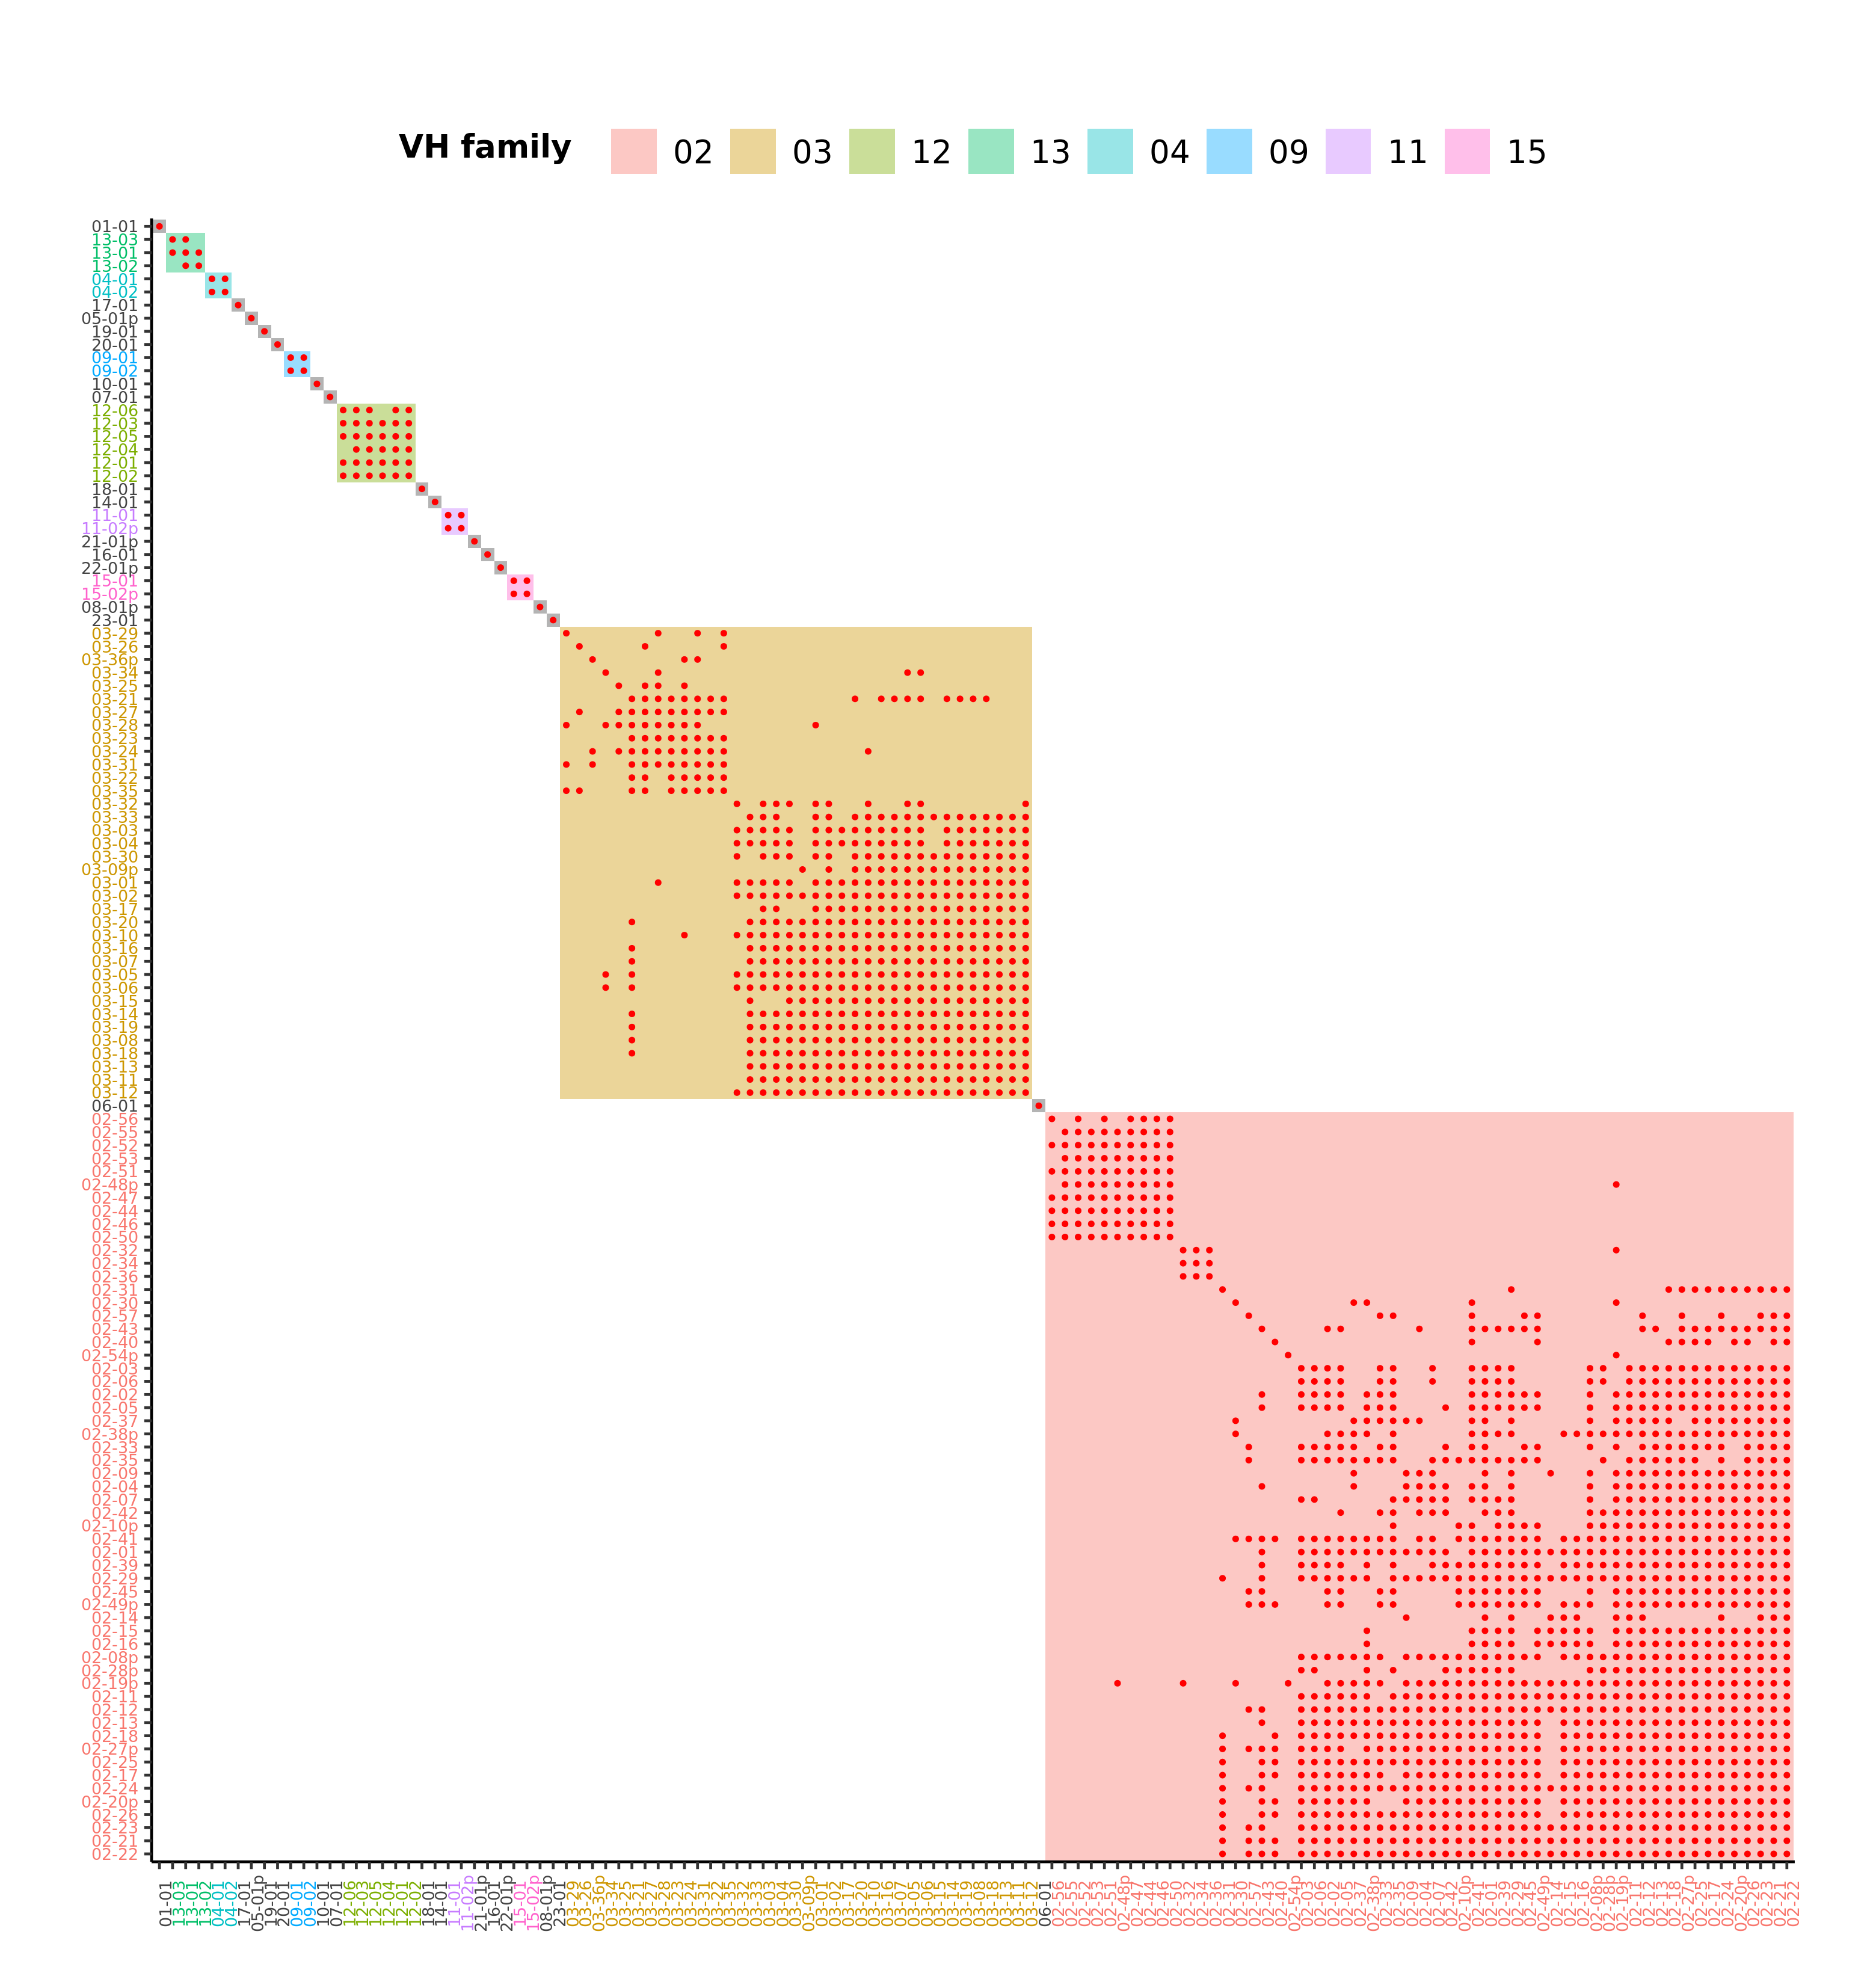
\includegraphics[width=\textwidth]{_Figures/png/xma-vh-families-map}
	\caption[Heatmap of \vh families in the in \Xma \textit{IgH} locus]{\textbf{Heatmap of \vh families in the in \Xma (\textit{IgH}) locus:} Heatmap of family relationships among \Xma \vh segments, with coloured shading indicating families and red dots indicating pairwise nucleotide sequence identity of at least 80\%. \vh families containing multiple segments are uniquely coloured, while single-segment families are in grey.}
	\label{fig:xma-vh-families-map}
	\end{figure}

	\begin{figure}
	\centering
	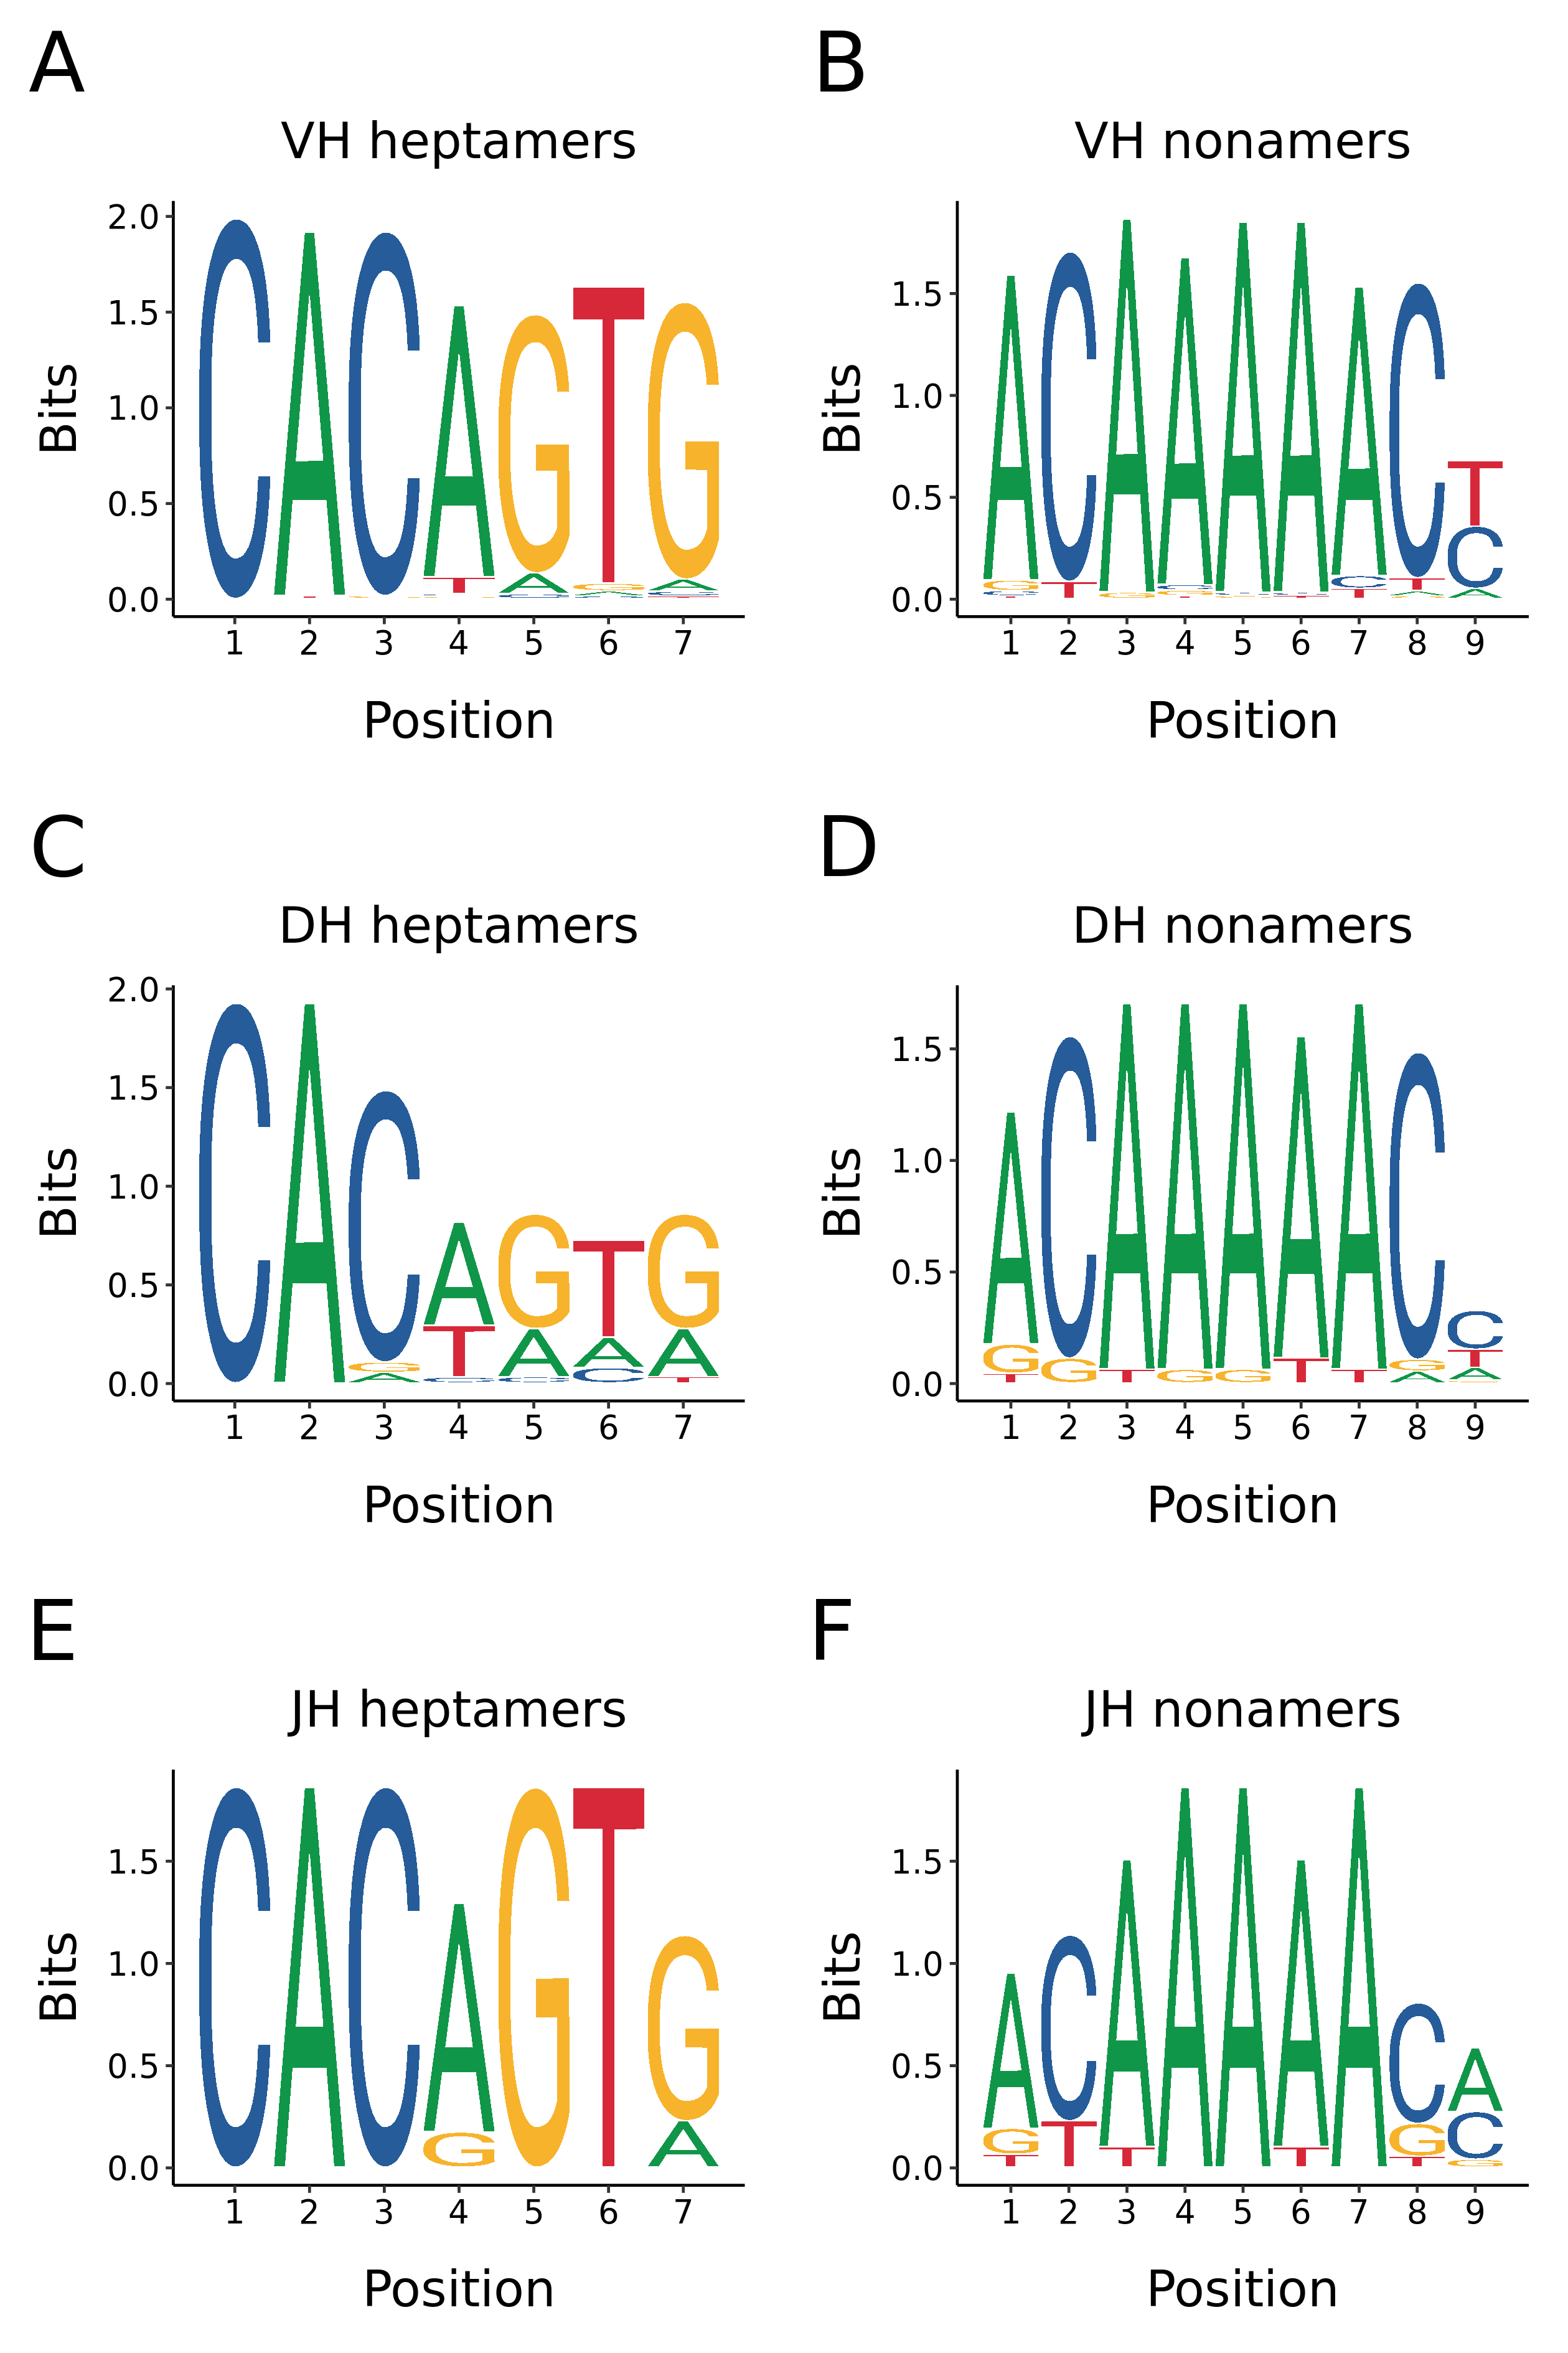
\includegraphics[width=0.9\textwidth]{_Figures/png/xma-new-rss-seqlogo-sep}
	\caption[\Xma recombination signal sequences by segment type]{\textbf{\Xma recombination signal sequences by segment type:} Sequence composition of conserved heptamer (A,C,E) and nonamer (B,D,F) sequences from \Xma heavy-chain RSSs associated with \vh (A,B), \dh (C,D) or \jh (E,F) gene segments.}
	\label{fig:xma-rss-seqlogo-sep}
	\end{figure}
	
% 4 - IGSEQ CHAPTER

\begin{figure}
\centering
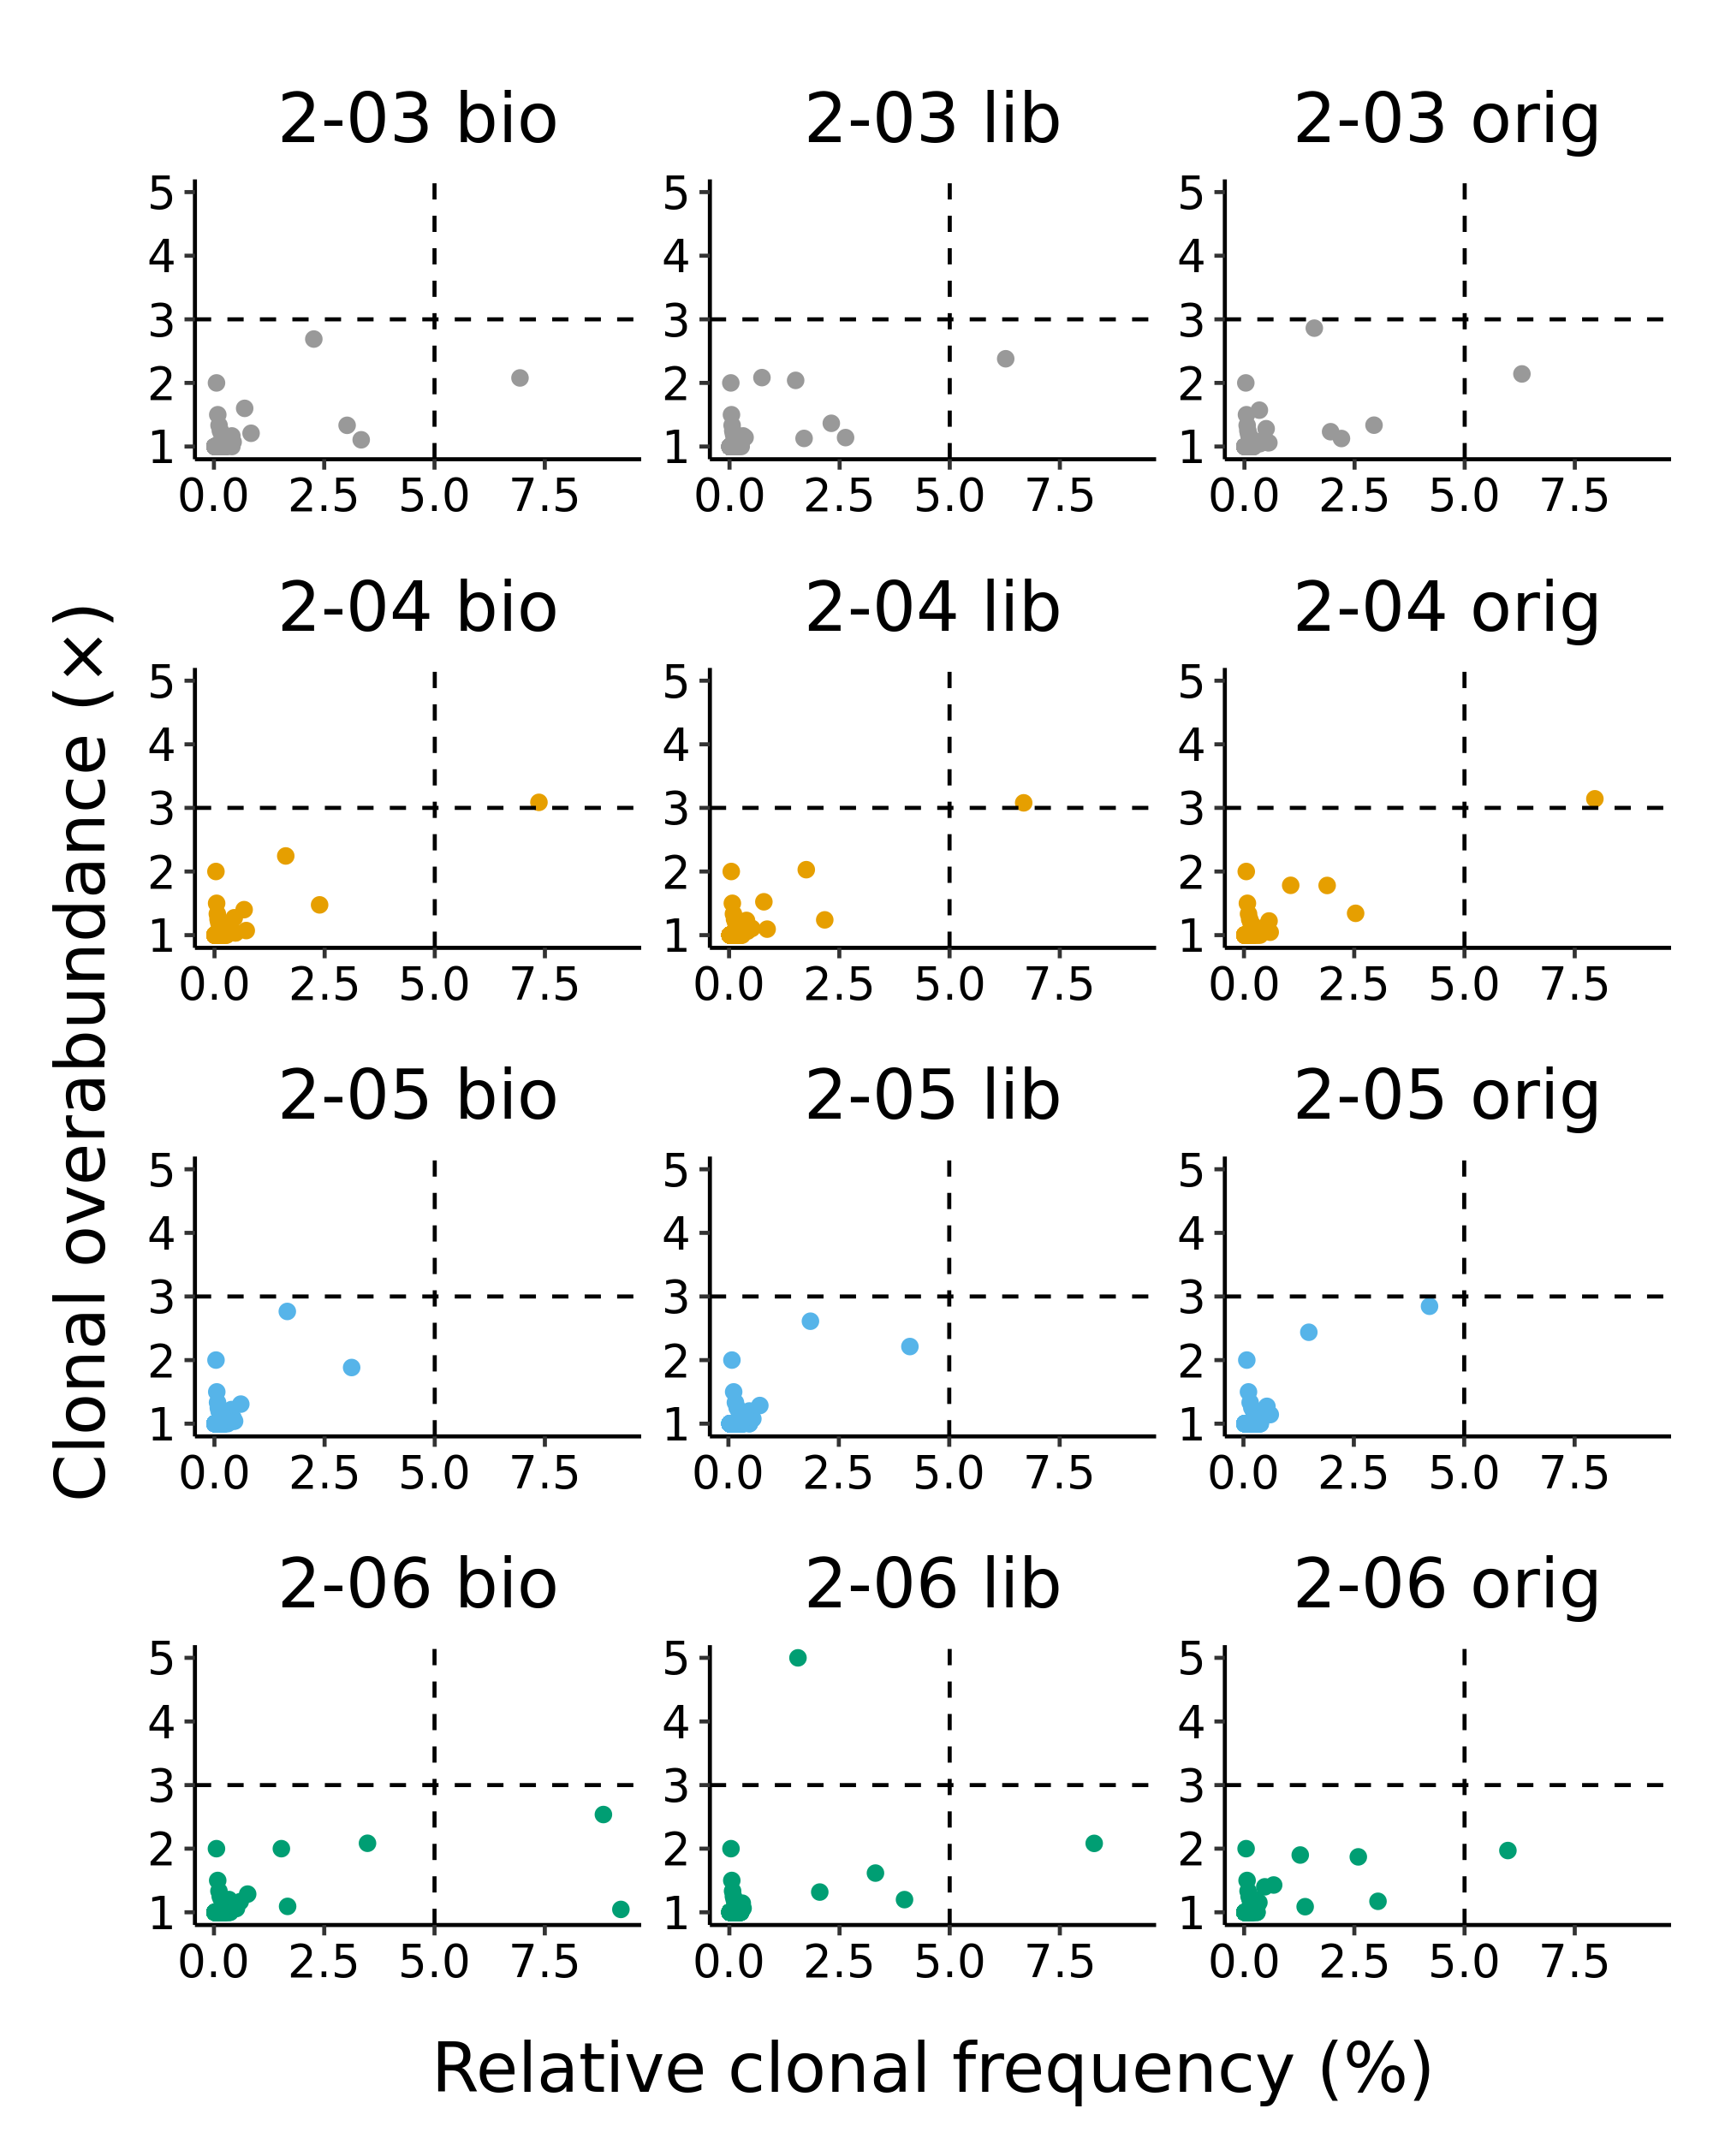
\includegraphics[width=0.8\textwidth]{_Figures/png/pilot-clones-expansions-rep}
\caption[Clonal expansions in \Nfu pilot repertoires]{\textbf{Clonal expansions in \Nfu pilot repertoires}: Scatter plots of clonal abundance for each replicate in the pilot \igseq dataset, measured in terms of the proportion of unique sequences in the repertoire ($x$-axis) and the abundance relative to the next-largest clone ($y$-axis). Thresholds for identifying clonal expansions (5\,\% and 3-fold for the $x$- and $y$-axis, respectively) suggested by Rosenfeld \textit{et al.} \parencite{rosenfeld2018clonesize}.}
\label{fig:igseq-pilot-clones-expansions-rep}
\end{figure} % TODO: Move to supplementary

\begin{figure}
\centering
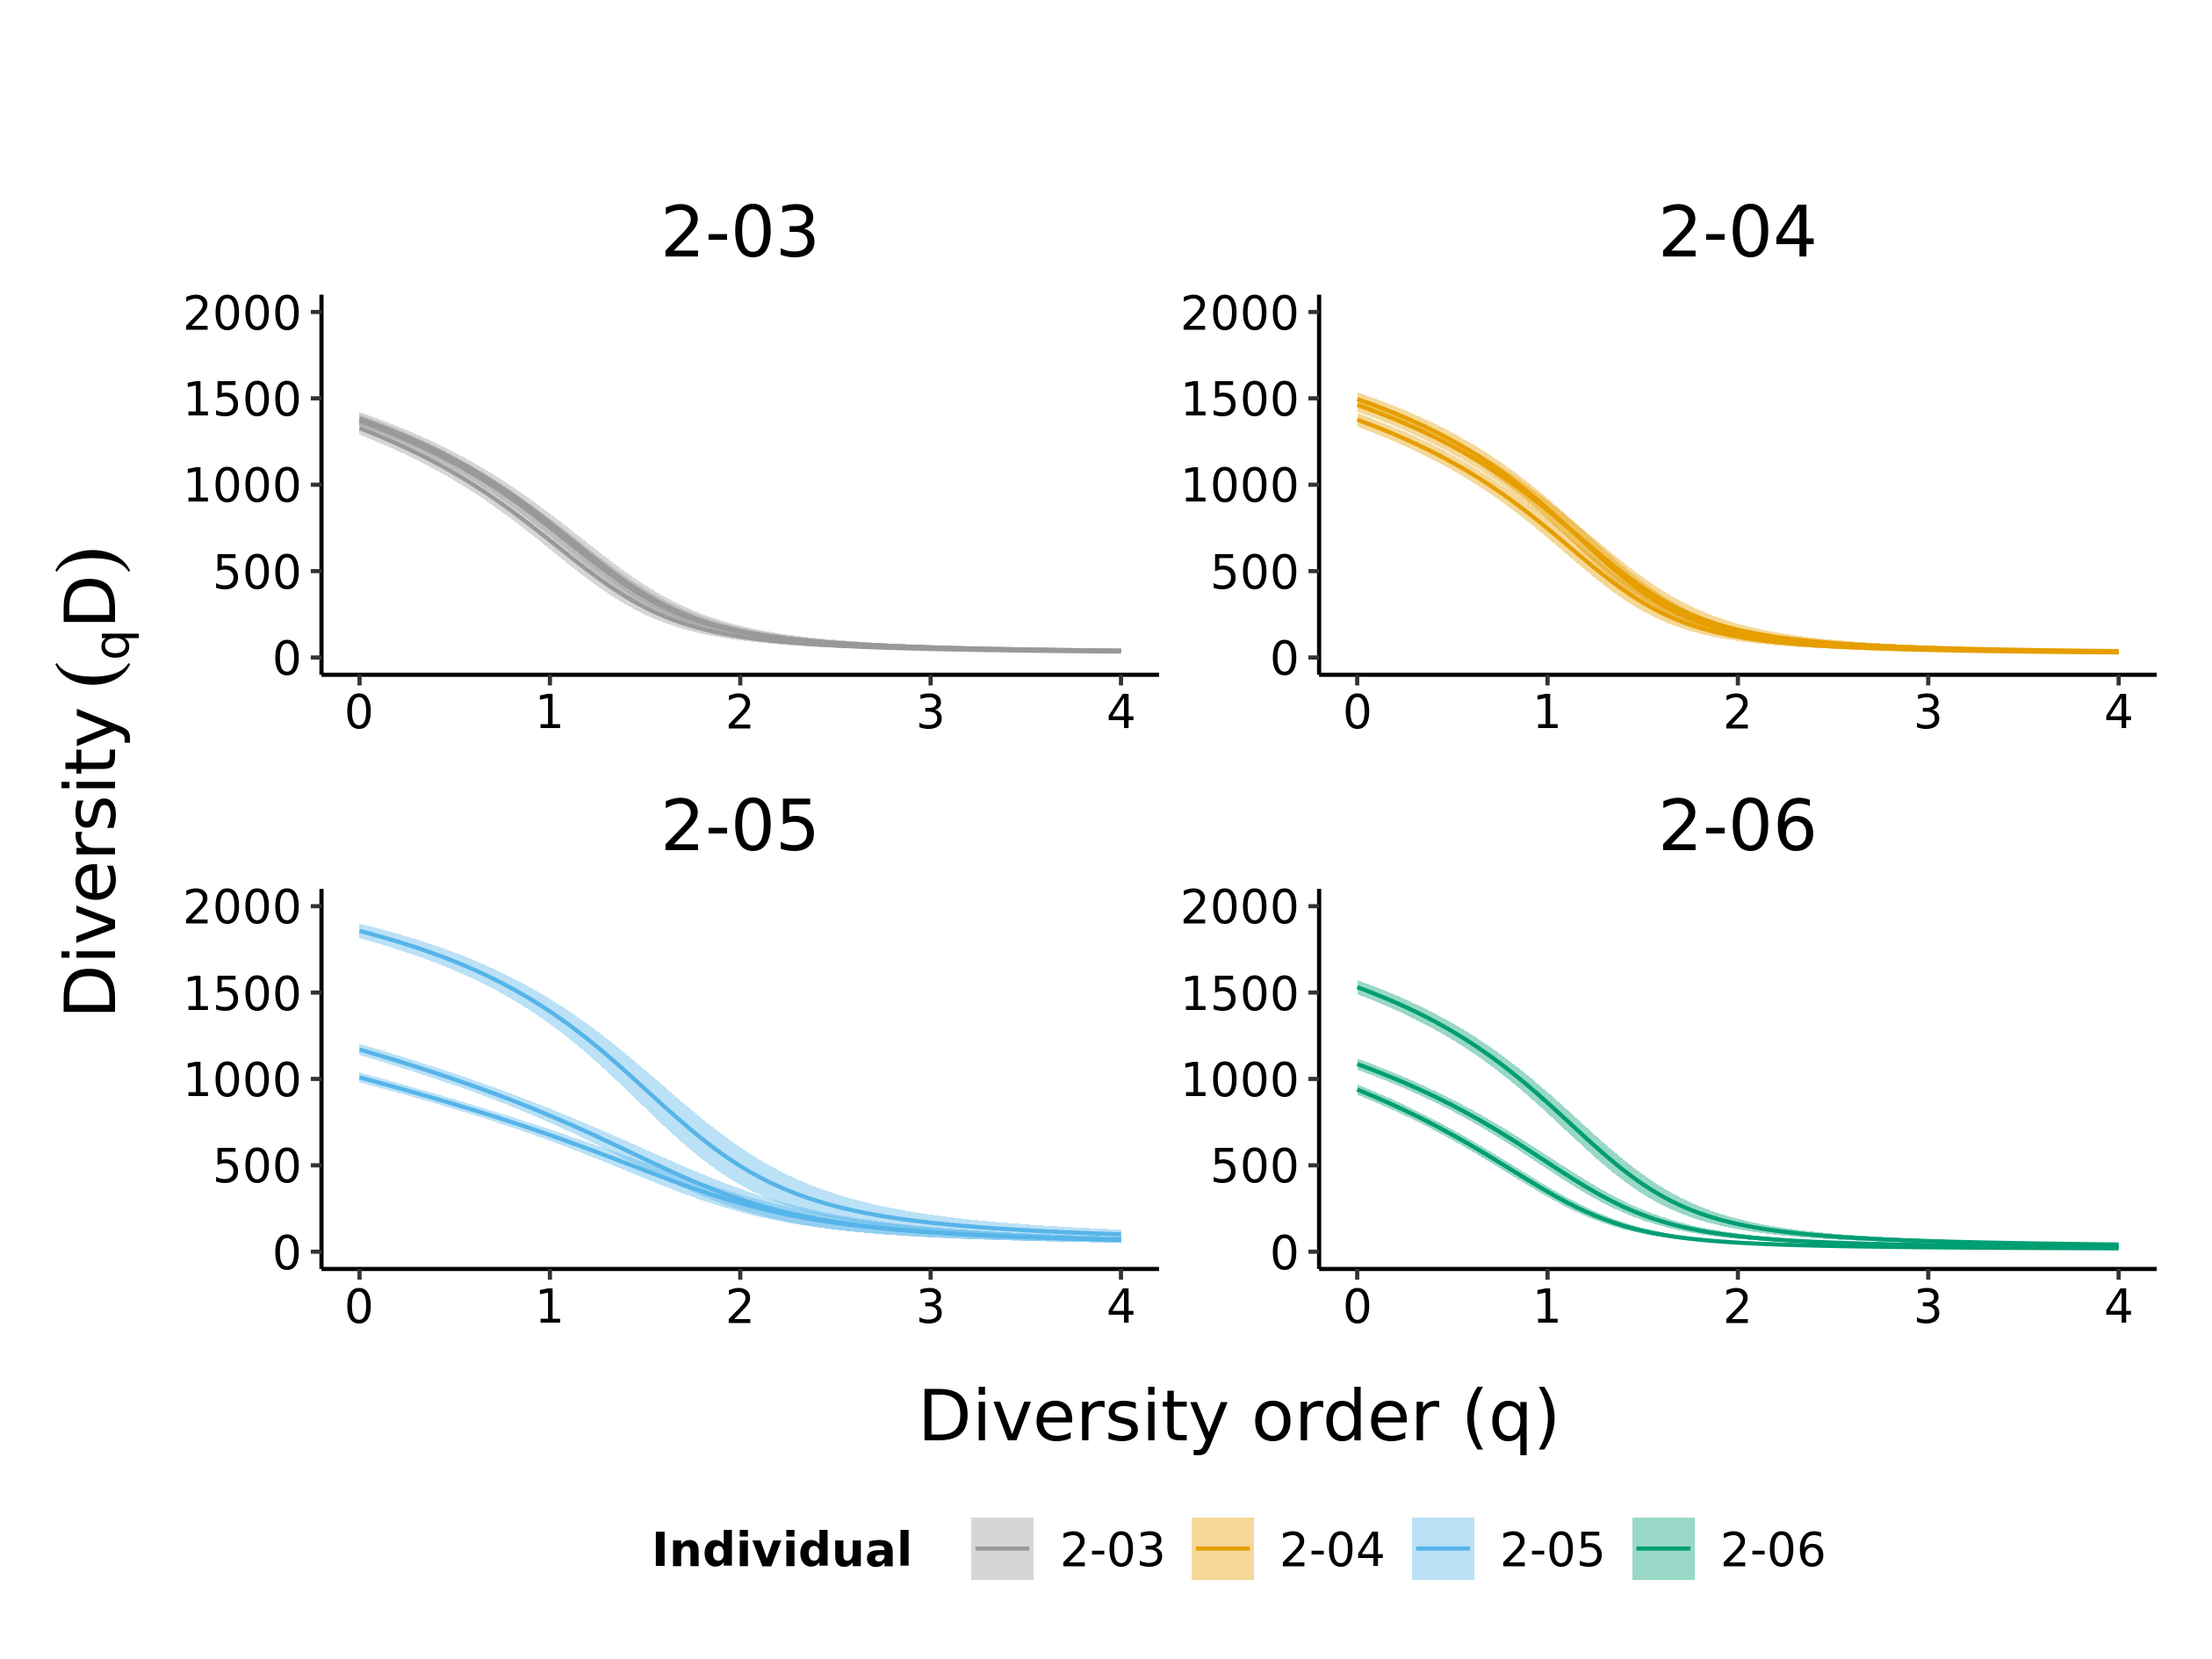
\includegraphics[width = 0.8\textwidth]{_Figures/png/pilot-clone-diversity-solo-spectra}
\caption{\textbf{Per-replicate clonal diversity for pilot dataset:} Hill diversity spectra of clone sizes (as measured by number of unique sequences per clone) for each replicate in the \igseq pilot dataset, grouped by source individual.}
\label{fig:igseq-pilot-clone-diversity-solo-spectra}
\end{figure} % TODO: Move to supplementary

\begin{figure}
\centering
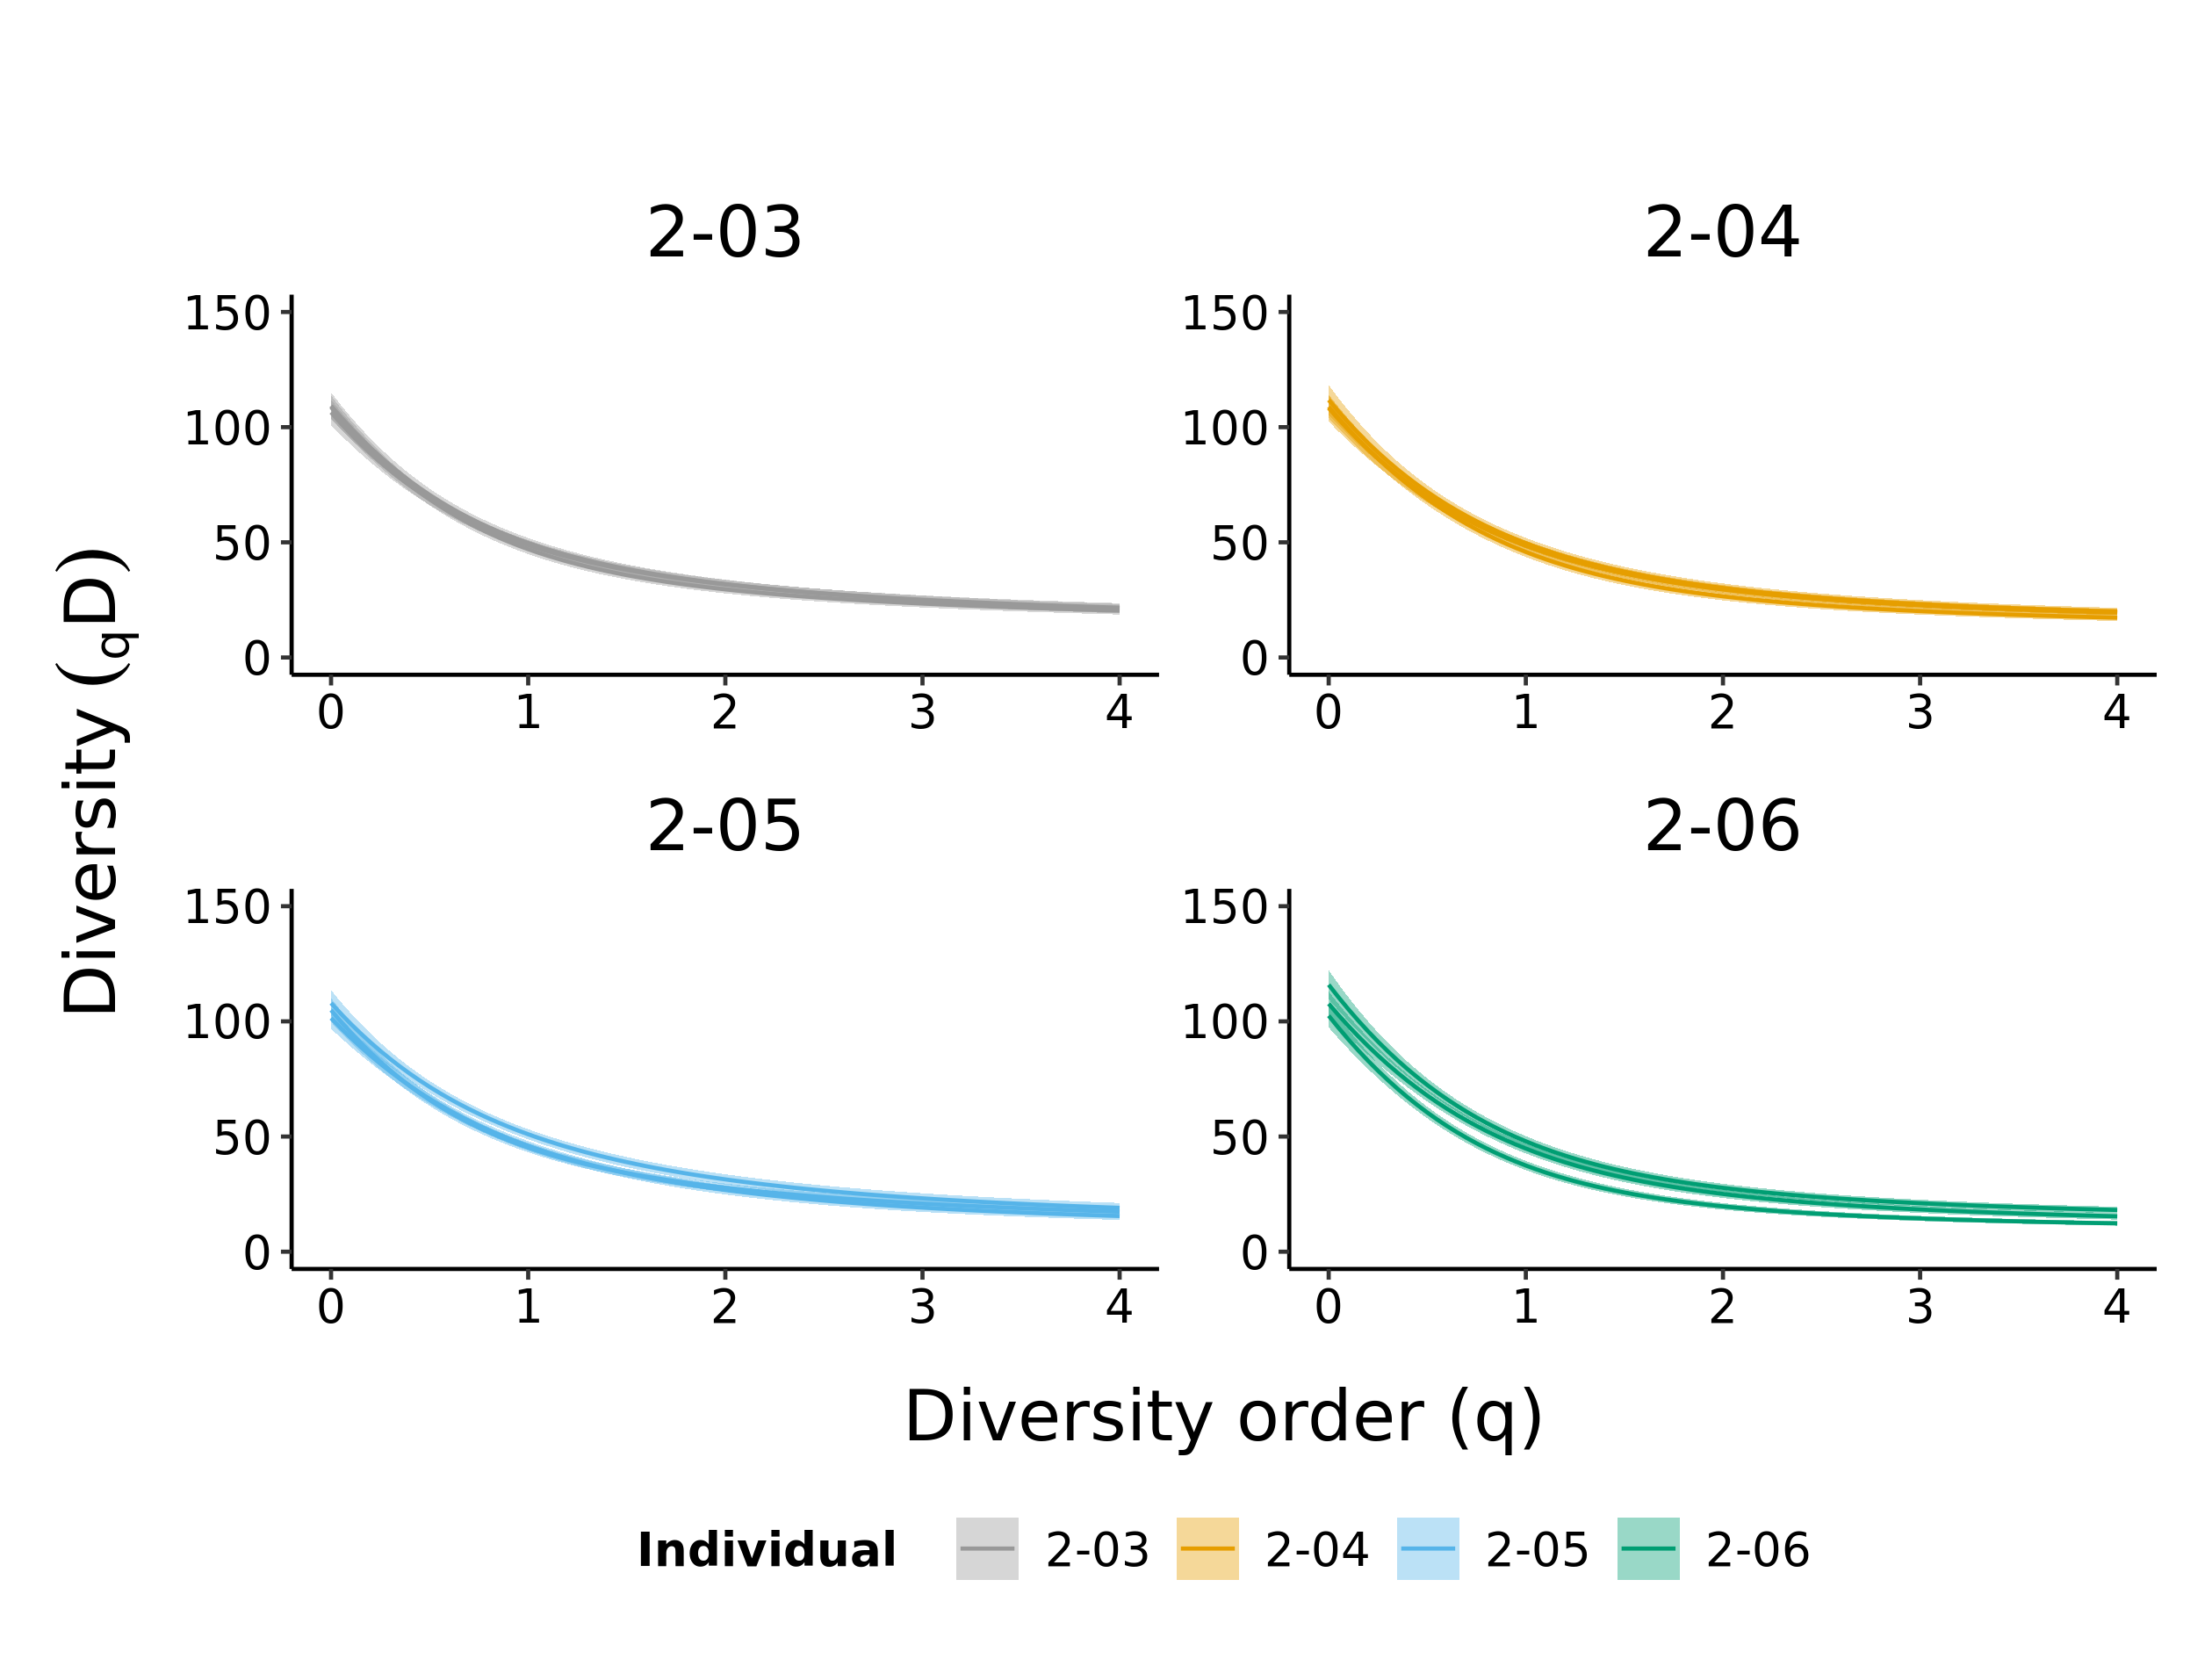
\includegraphics[width = 0.8\textwidth]{_Figures/png/pilot-vj-diversity-solo-spectra}
\caption{\textbf{Per-replicate VJ-diversity for pilot dataset:} Hill diversity spectra of VJ usage (as measured by number of unique sequences per V/J combination) for each replicate in the \igseq pilot dataset, grouped by source individual.}
\label{fig:igseq-pilot-clone-diversity-vj-spectra}
\end{figure} % TODO: Move to supplementary

\begin{figure}
\centering
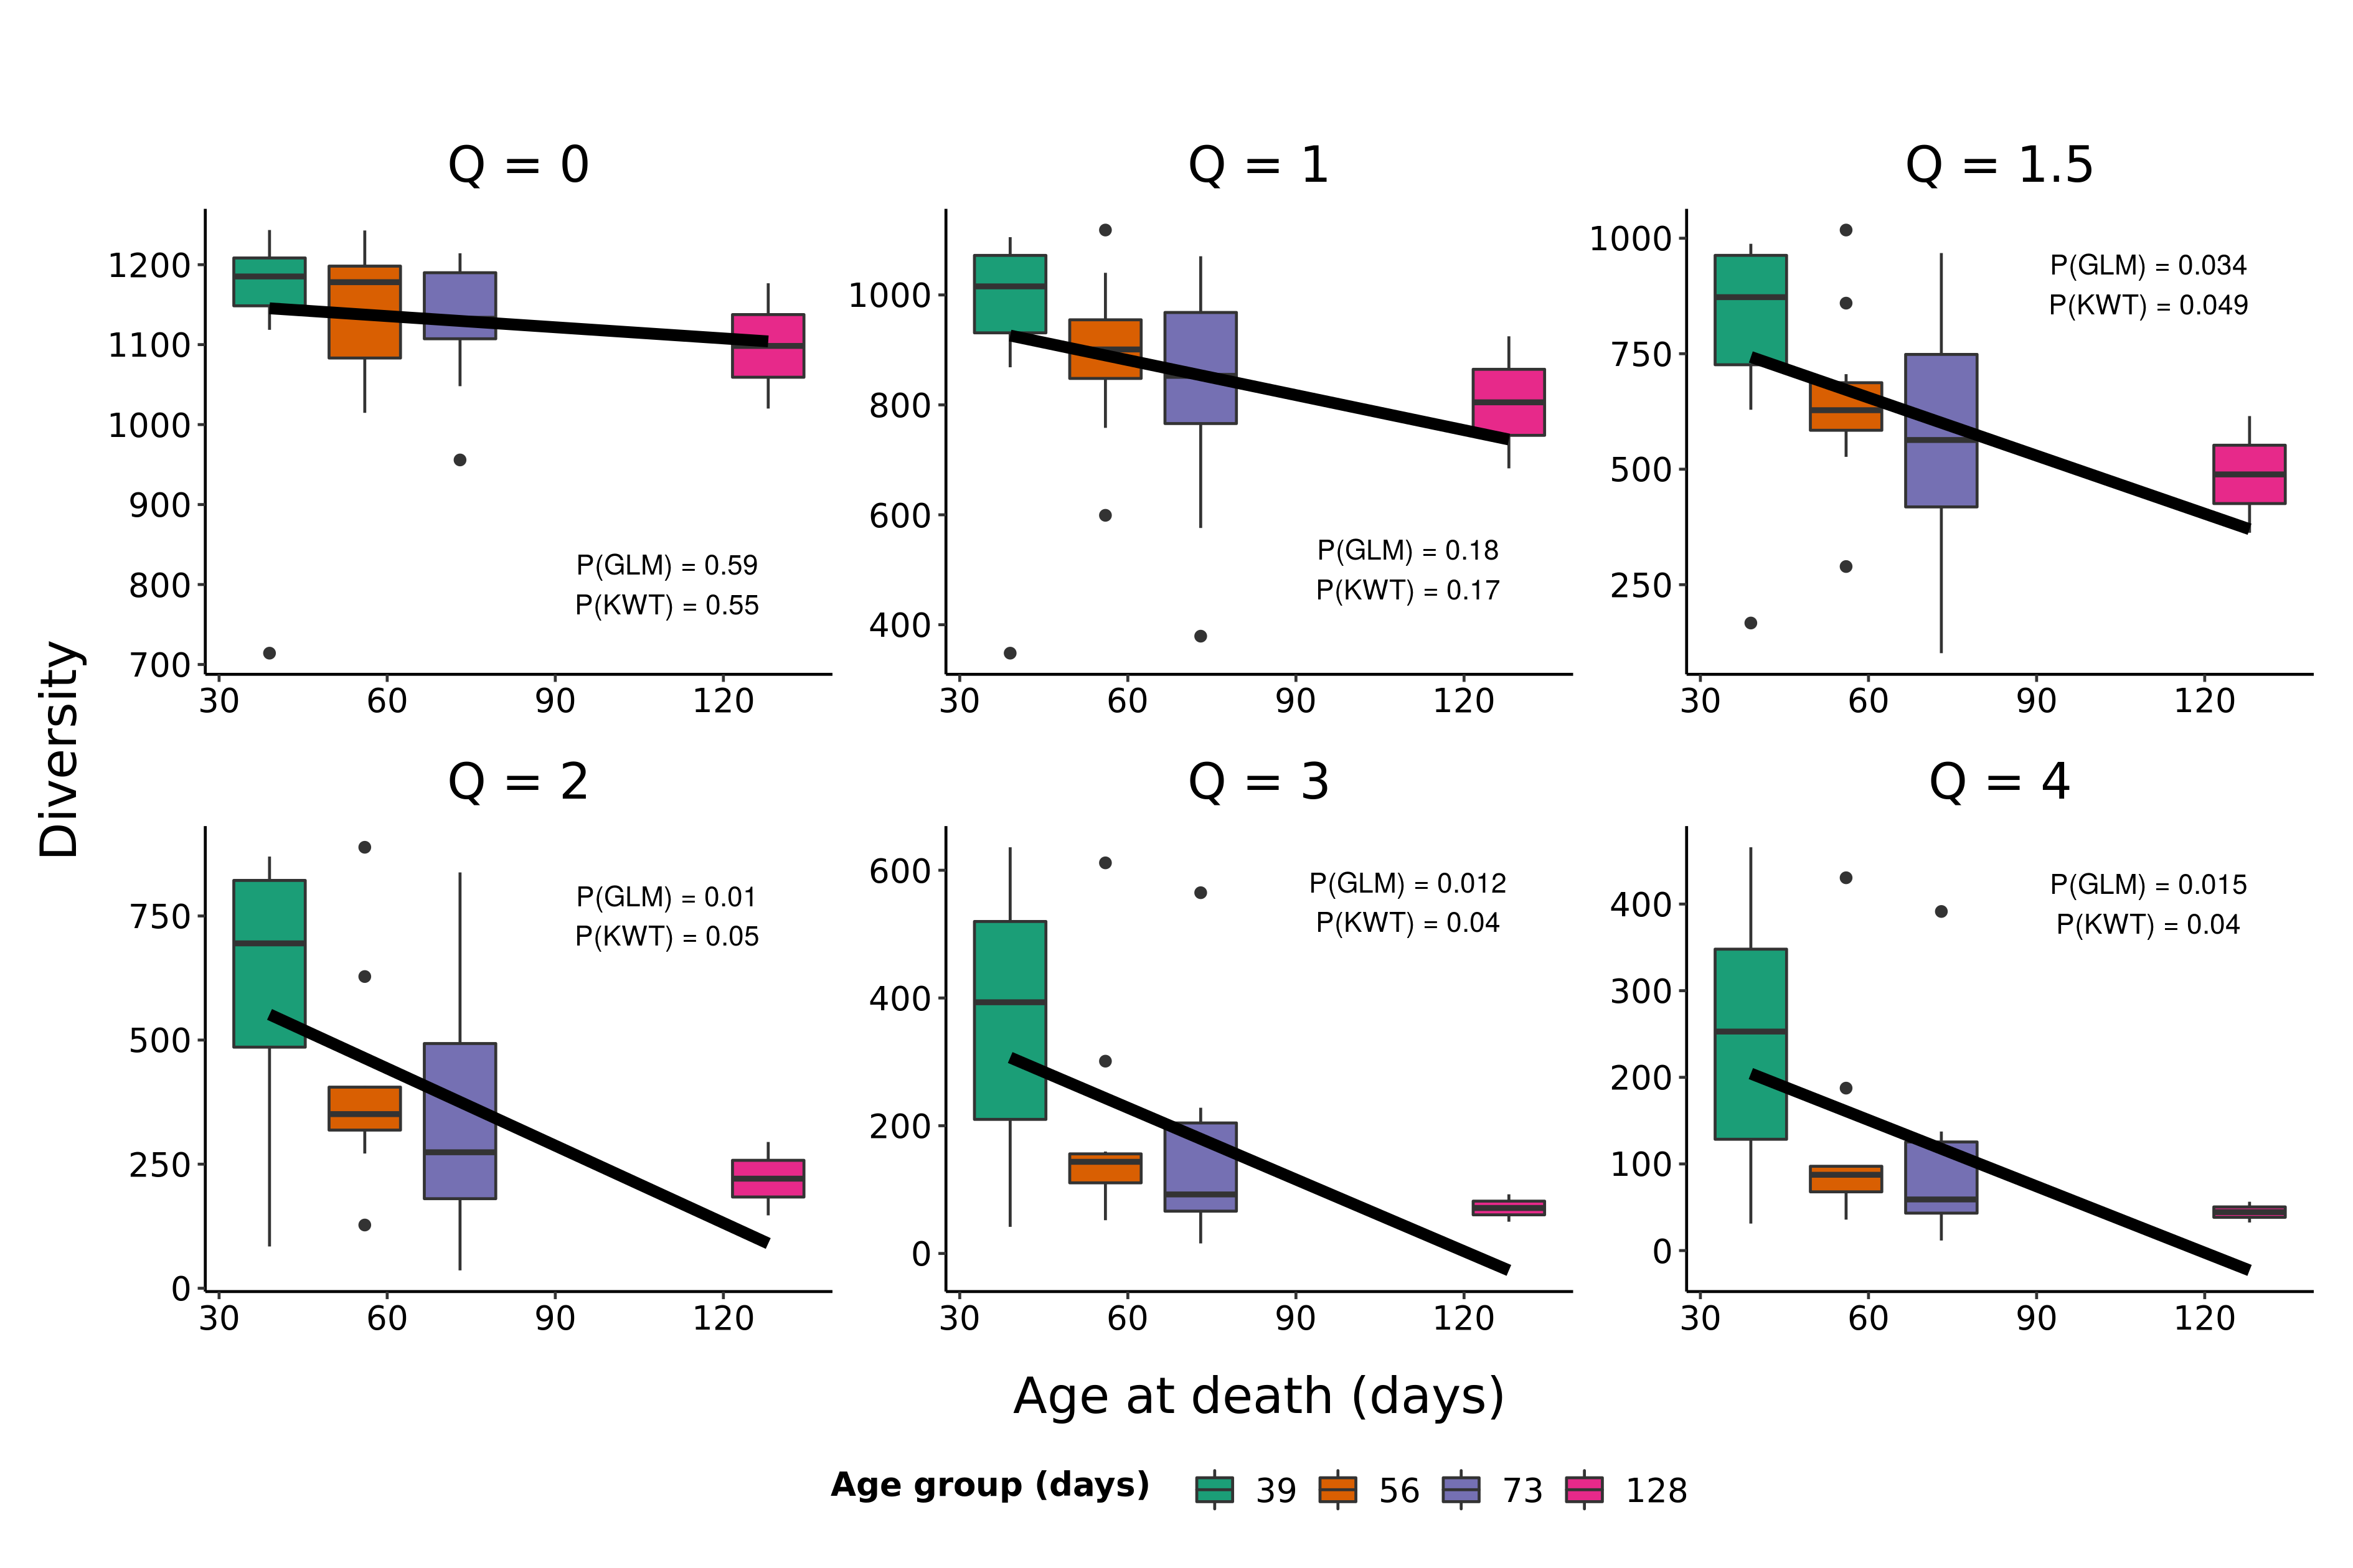
\includegraphics[width = 0.9\textwidth]{_Figures/png/ageing-clone-diversity-solo-fit-linear}
\caption{Boxplots of Hill diversity values for the antibody repertoires of individuals of each age group in the \igseq ageing dataset at a sample of diversity orders, overlaid with the predictions of the best-fit linear model at each order.}
\label{fig:igseq-ageing-clone-diversity-solo-fit-linear}
\end{figure}

\begin{figure}
\centering
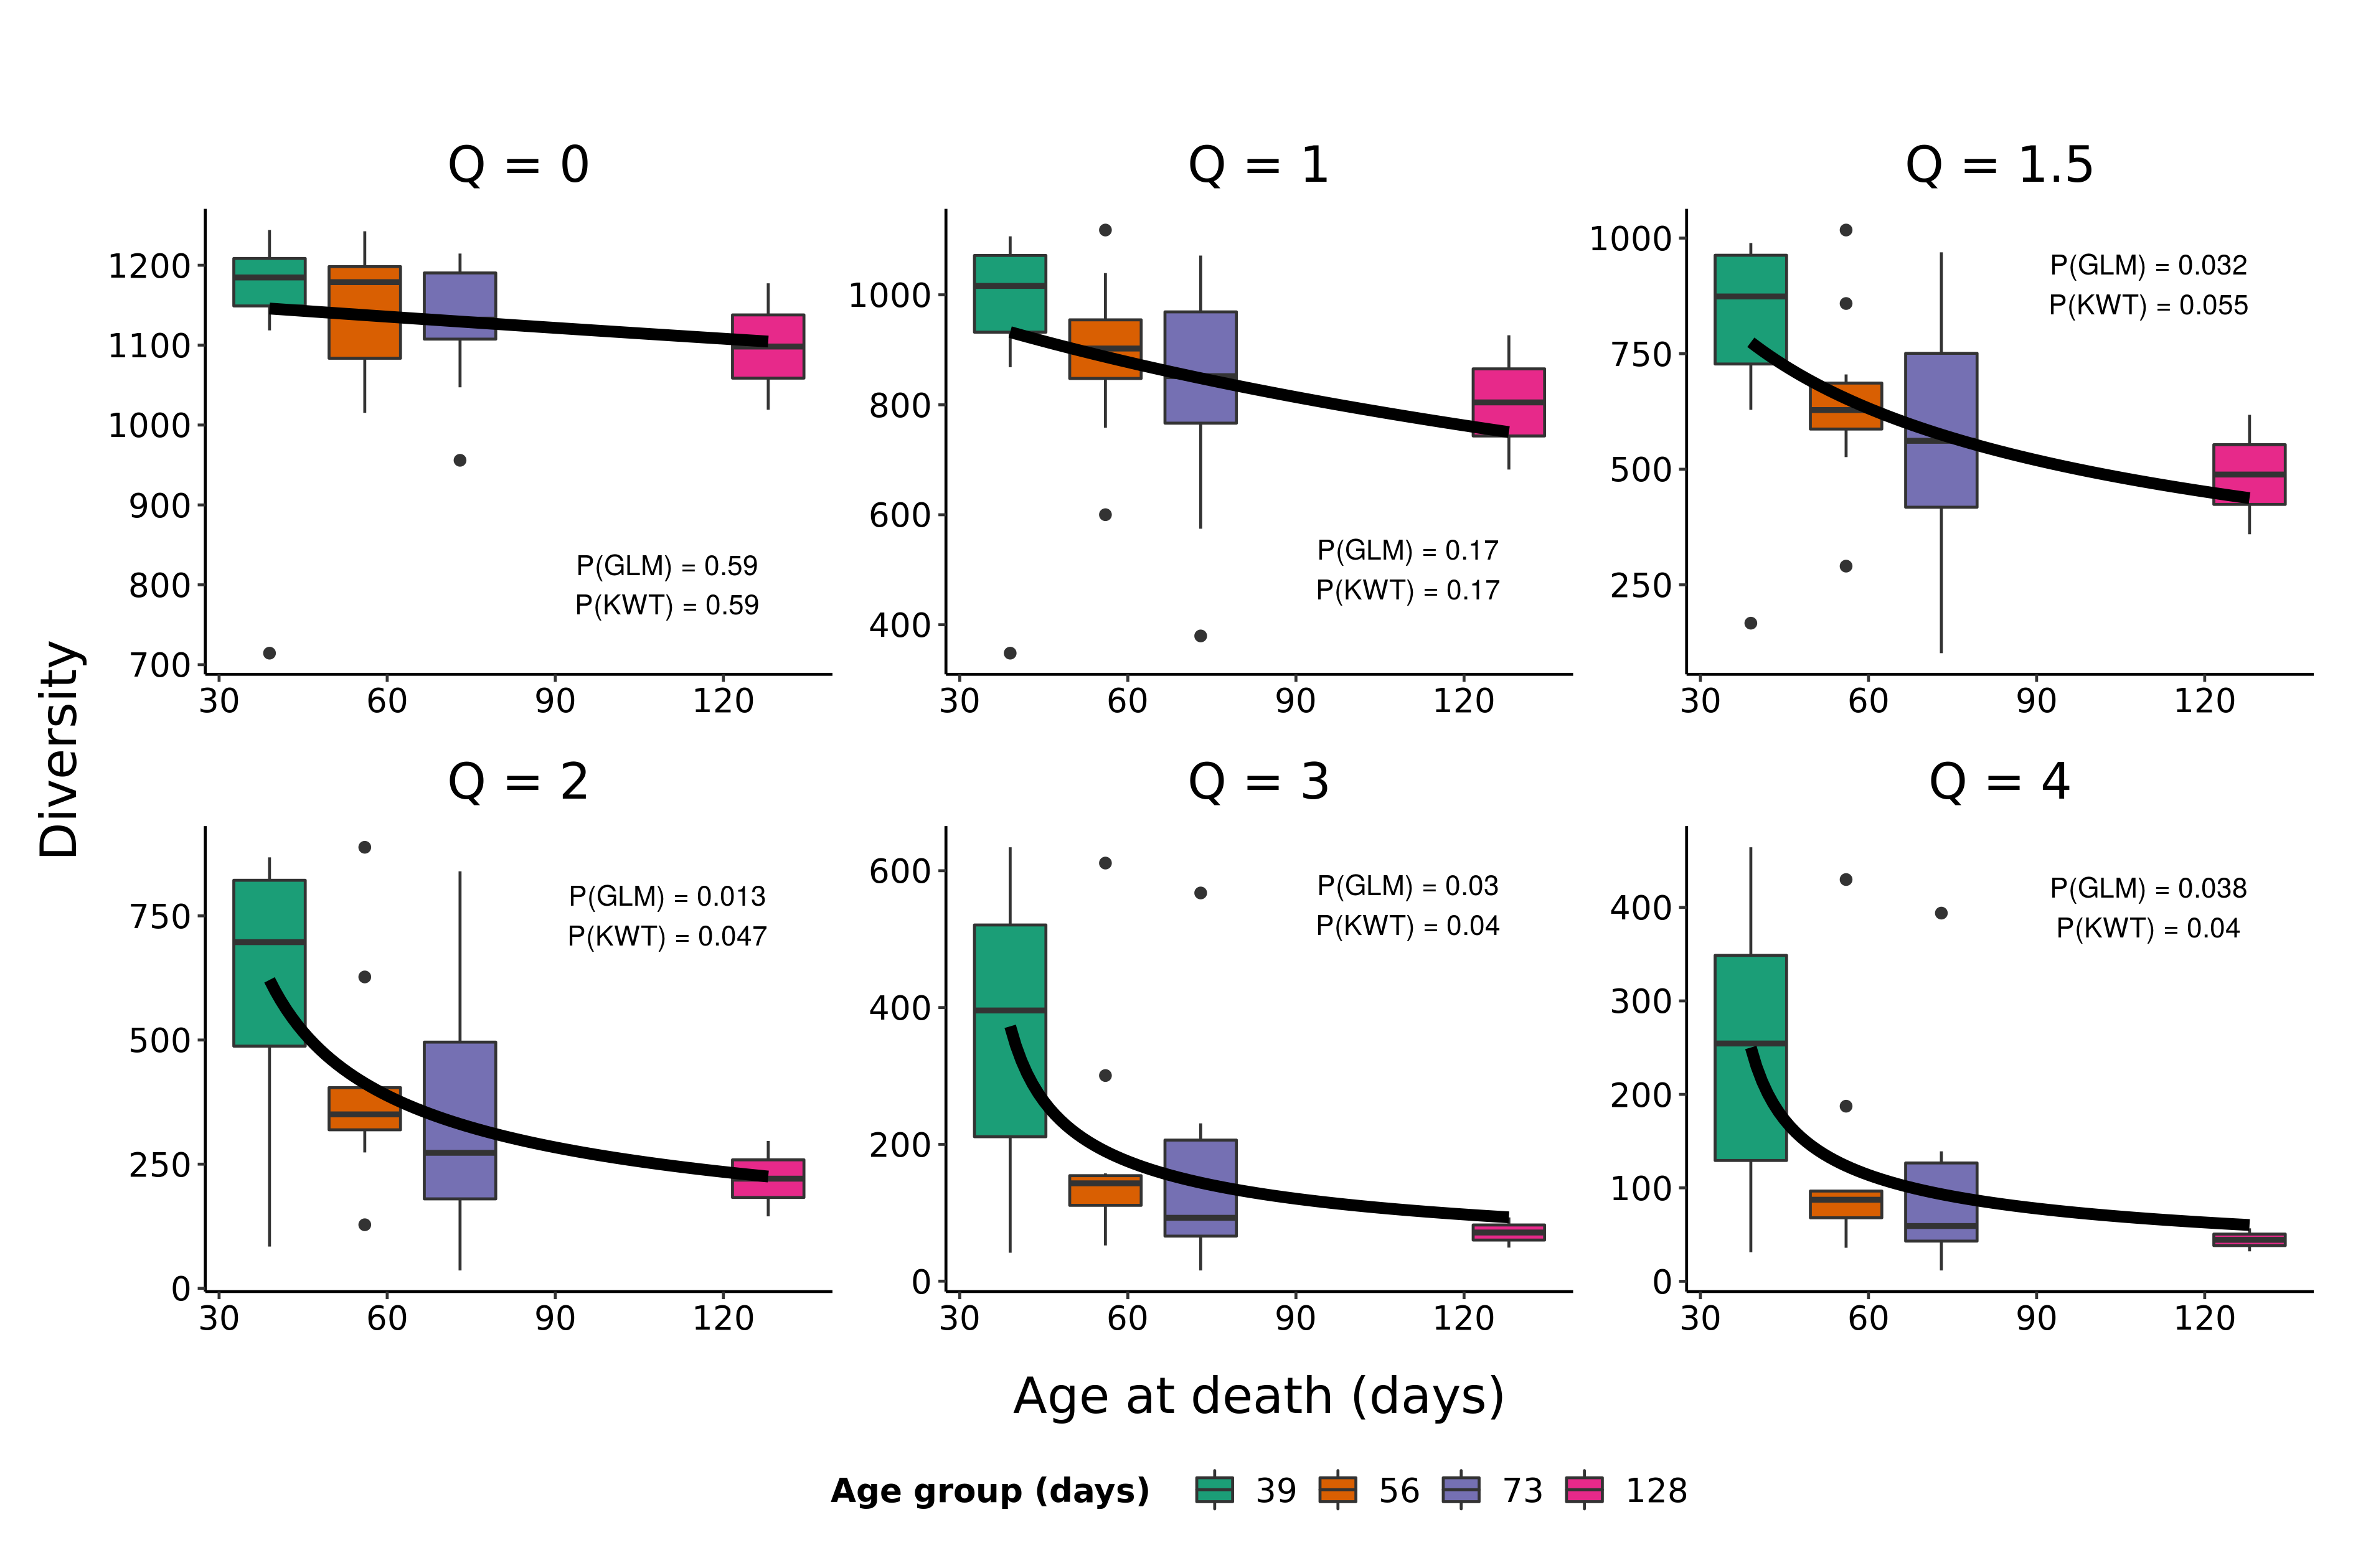
\includegraphics[width = 0.9\textwidth]{_Figures/png/ageing-clone-diversity-solo-fit-igauss}
\caption{Boxplots of Hill diversity values for the antibody repertoires of individuals of each age group in the \igseq ageing dataset at a sample of diversity orders, overlaid with the predictions of the best-fit inverse-Gaussian-distributed GLM at each order.}
\label{fig:igseq-ageing-clone-diversity-solo-fit-igauss}
\end{figure}

\begin{figure}
\centering
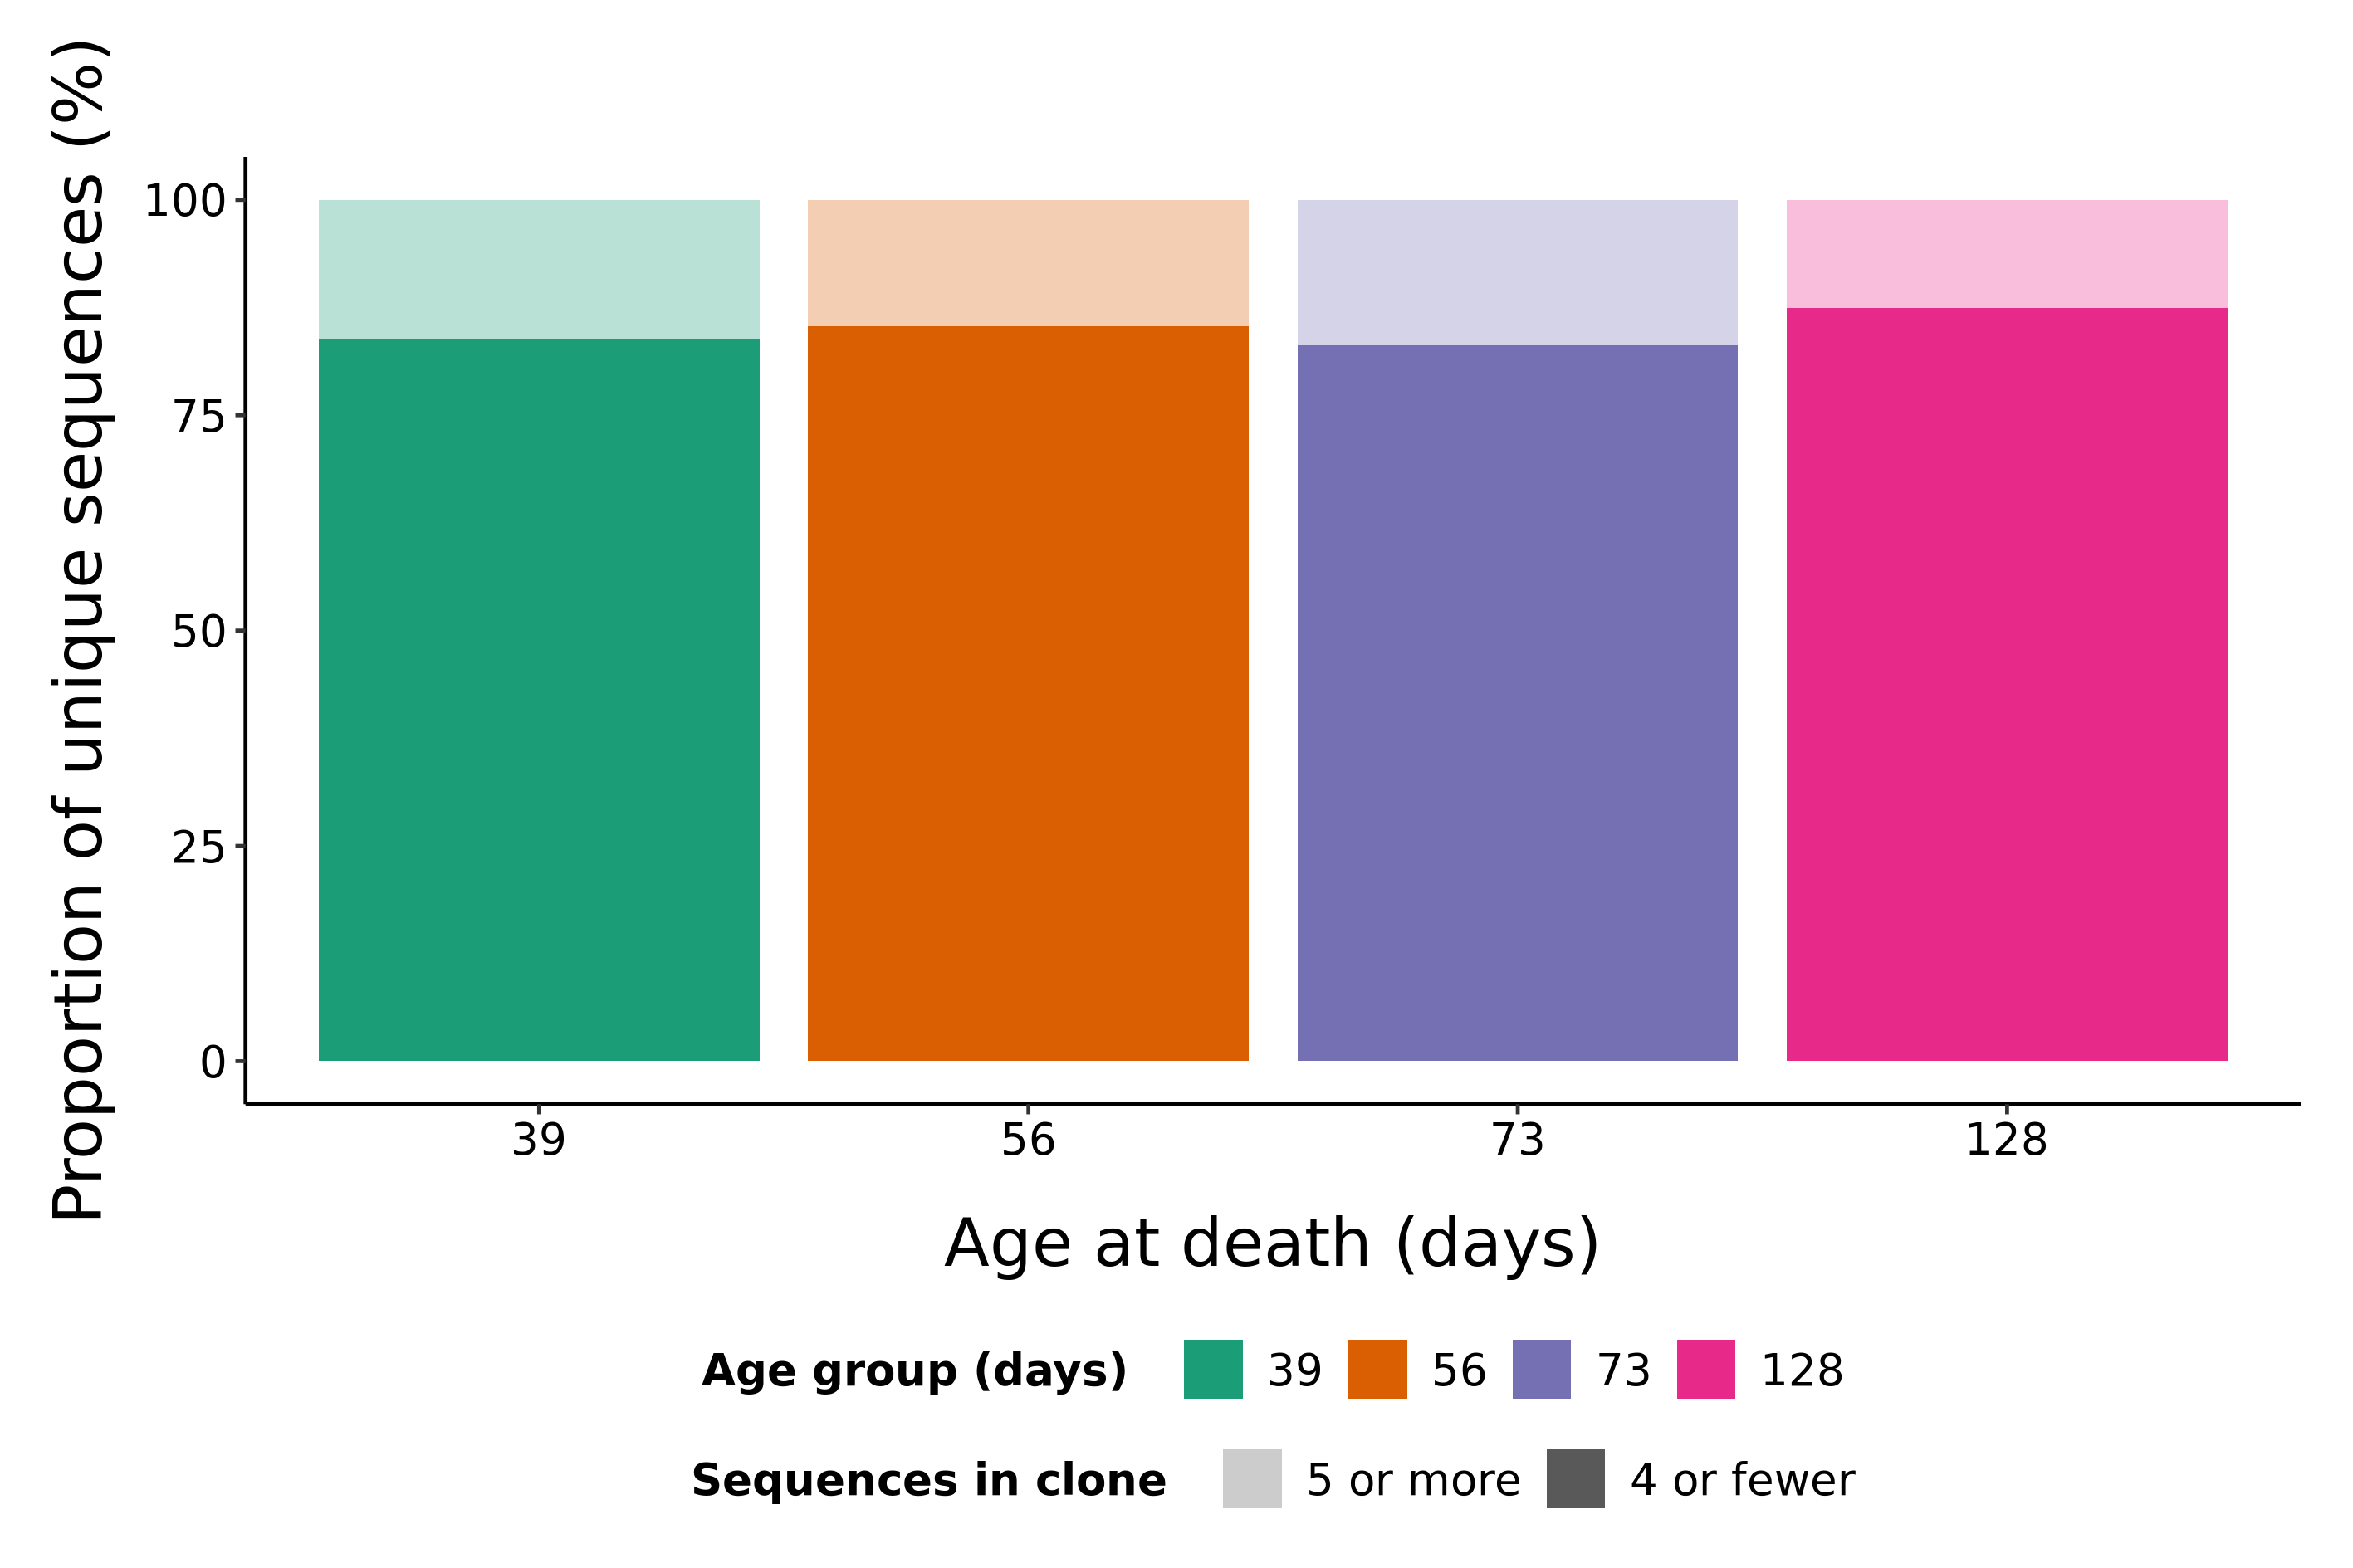
\includegraphics[width = 0.9\textwidth]{_Figures/png/ageing-pc-seq-in-small-clones}
\caption[Proportion of unique sequences in small clones in the \igseq ageing dataset]{\textbf{Proportion of unique sequences in small clones in the \igseq ageing dataset:} Stacked barplots of average proportion of abundant (5 or more unique sequences, top, pale) vs non-abundant (4 or fewer, bottom, dark) in each age group in the \igseq ageing dataset. The proportion of non-abundant clones does not change significantly with age (Kruskal-Wallis analysis of variance, $p=\embed{_Figures/txt/ageing-pc-seq-in-small-clones-kruskal-p.txt}$).}
\label{fig:igseq-ageing-pc-seq-in-small-clones}
\end{figure}